% !TEX TS-program = lualatexmk
\def\fsc{11pt}
\documentclass[\fsc]{article} 
\usepackage[margin=1in]{geometry} 
\usepackage[parfill]{parskip}
%\pdfmapfile{=newtx.map}

%\pdfcompresslevel=0
%\pdfgentounicode=1
%\input glyphtounicode.tex
%\usepackage{pdfx} % v 1.6.4 or higher
%\InputIfFileExists{glyphtounicode-cmr.tex}{}{}
%\InputIfFileExists{glyphtounicode-ntx.tex}{}{}
\usepackage{graphicx} 
\usepackage{url}
\usepackage{trace}
\usepackage{fonttable}
%\usepackage[debugshow]{tracefnt}
\usepackage{xcolor}
\usepackage{array,booktabs}
% some ad-hoc symbol fonts
\font\fAMSa=msam10 at \fsc
\font\fAMSb=msbm10 at \fsc
\font\ebgmi=ntxebgmi at 11.5pt
%\pdfmapfile{=newtx.map}
\usepackage[T1]{fontenc} % Active encoding for use in math text
%\renewcommand{\rmdefault}{minntx}% Roman and Bold Termes for math
\usepackage[type1,sfdefault,scale=1]{sourcesanspro}% used by \mathsf, optional
\usepackage[scaled=.98,varqu,varl]{zi4}
%\usepackage[amsthm,largesc,theoremfont,trueslanted,scosf]{newtx}% Use newtxmath, not a unicode math package
\usepackage[amsthm,theoremfont,newsu,scosf]{newtx}% Use newtxmath, not a unicode math package
%\usepackage{amsthm}
%\usepackage{newtxmath}
%\usepackage[largesc,theoremfont,scosf]{newtxtext}
%\usepackage[no-math]{fontspec}
%\setmainfont{TeXGyreTermesX}
%\setsansfont{sourcecodepro}[scale=MatchLowerCase]
\makeatletter
\@ifundefined{ver@amsthm.sty}{\typeout{amsthm NO}}{\typeout{amsthm YES}}
\makeatother
%theorem settings
\newtheoremstyle{oldplain}
  {\topsep}   % ABOVESPACE
  {\topsep}   % BELOWSPACE
  {\itshape}  % BODYFONT
  {}       % INDENT (empty value is the same as 0pt)
  {\bfseries} % HEADFONT
  {.}         % HEADPUNCT
  {5pt plus 1pt minus 1pt} % HEADSPACE
  {}          % CUSTOM-HEAD-SPEC
\theoremstyle{oldplain}
\newtheorem{oldthm}{Theorem}[section]
\theoremstyle{plain}
\newtheorem{thm}{Theorem}[section]
% ed theorem settings 
\DeclareMathSymbol{\bbZ}{\mathord}{lettersA}{218}
\DeclareMathSymbol{\Sumop}{\mathop}{largesymbols}{"50}
\usepackage{bm}
%\usepackage{hyperref}
%\iftutex
%	\setmonofont{inconsolata}[Scale=MatchLowercase]
%\fi
\title{New TX font package}
\author{Michael Sharpe}
\date{\today}  % Activate to display a given date or no date
\begin{document}
\makeatletter
%\expandafter\show\csname @textsuperior\endcsname
%\expandafter\show\csname opt@libertine.sty\endcsname
\makeatother
%%\show\textsfrac
%\show\ntx@TF
%\makeatother
\maketitle
%\char"2044{\addfontfeatures{RawFeature=+ss20;+dnom}\color{red}\char"2044}
%1\addfontfeatures{VerticalPosition=Inferior}23
%{\itshape italic:;}
%\textcircled{M}\textcircled{12}\textfrac[2]{37}{78}
%\font\inf=ntxinf-Regular-t1 at \fsc
%1{\infigures 1}
%x\textsf{x}X\textsf{X}
%
\section{Introduction}
This package is meant to be a replacement for Young Ryu's {\tt txfonts}. It is  a complete text ({\tt newtxtext}) and math ({\tt newtxmath}) package with roman text font provided by  a Times clone, sans serif based on a \textsf{Helvetica} clone, typewriter faces, plus math symbol fonts whose math italic letters are from a Times Italic clone. As of version 1.4, {\tt newtxtext} no longer depends on {\tt txfonts} but is based on the richer source \textsf{TeXGyre Termes}, but {\tt newtxmath} continues to use the {\tt txfonts} math glyphs with many metric adjustments and some wholesale modifications.

\textsc{Changes as of version 1.735}
\begin{itemize}
\item
If {\tt newtx} or {\tt newtxtext} detects that a prior package loaded {\tt fontspec}, then it avoids trying to reload it. While this reduces the risk of an {\tt option clash error}, it means that the prior package will have complete resposibility for loading {\tt fontspec} with an option to control its math handling, specifically {\tt no-math}. For example, if using the {\tt xeCJK} package together with {\tt newtxtext.sty} and {\tt newtxmath.sty}, a minimal preamble could be something like:
\begin{verbatim}
\PassOptionsToPackage{no-math}{xeCJK}
\documentclass{ctexart}
\setCJKmainfont{SimSun}
\usepackage{newtx}
\end{verbatim}
or
\begin{verbatim}
\documentclass{article}
\usepackage[no-math]{xeCJK}
\setCJKmainfont{SimSun}
\usepackage{newtx}
\end{verbatim}
\item Because options {\tt no-math} and {\tt otfmath} were mentioned in previous versions of the documentation, I've kept both in the current version even though not logically necessary as one is the negation of the other. In fact, if both are specified, or, equivalently, both are set equal to {\tt true}, then {\tt otfmath wins}.
\end{itemize}

\textsc{Changes as of version 1.73}
\begin{itemize}
\item
Superior letters and figures distinct from numerators have been added along with some special features. The text switch \verb|\sustyle| (or \verb|\sufigures|) or the commands \verb|\textsu|, \verb|\textsup|, \verb|\textsups| may be used to invoke ordinary superiors. 
The command \verb|\textsuperscript| is reserved for a form of superiors that respond to adjustments you may specify in the package options, and which are used for footnote marker typesetting: \verb|supscale| rescales them, \verb|supsraised| specifies an amount to move them vertically, and \verb|supLspaced|, \verb|supRspaced| specify additional kerning to be applied at the left and right. These changes are applied in the order: scaling, raising, kerning.  All except \verb|supscale| should be dimensions with units like {\tt em} which will scale properly. Their relative vertical positions stack up like this: X\textinf{12}X\textde{345}X\textnu{678}X\textsu{90}.
 There is also a {\tt supscolor} option that will apply a color specified in a form understood by {\tt xcolor}, like {\tt red!70!black}. \textbf{IMPORTANT: As of version 1.737, the options and code described in this paragraph has been moved to the new completely rewritten  {\tt superiors} package.}
\item 
Version 1.732 introduces some new mathematical glyphs. First,  there are new curly braces invoked by the option {\tt curlybraces} with {\tt height+depth} of 940, 1200, 1800, 2400, 3000 and 3600 em units. Second, there are three new math symbols:
\begin{itemize}
\item
\verb|\laplace|, $\laplace$, which is an inverted \verb|\nabla|, having more weight in the  bottom segment than \verb|\Delta|, $\Delta$.
\item
\verb|\laplac|, $\laplac$. This is the unicode-math name for the official d'Alembertian operator, {\tt U+29E0}. Unlike  $\laplace$, it has more weight in the left and top segments than \verb|\laplace|.
\item \verb|\dAlembertian|, $\dAlembertian$, rotates $\laplac$ by 180${}^\circ$, making for a glyph whose weight distribution is a better match for the Laplacian.
\end{itemize}
% \item A word of warning---there is a difference between XeLaTeX and LuaLaTeX that is very irritating. When processing some of the commands where there may be a numeric argument, such as, for example,  \verb|{\addfontfeature{VerticalPosition=Superior}5}|, the output will be as expected with XeLaTeX but not with LuaLaTeX if you have set the document figures to be anything but the default tabular, lining. This happens even though the {\tt sups} table has entries for all other forms ({\tt oldstyle}, {\tt taboldstyle} and {\tt lining}) of main body figures, and the {\tt sups} lookup is ahead of the {\tt lnum}, {\tt tnum}, {\tt onum} and {\tt pnum} lookups. (Similarly for the {\tt subs}, {\tt numr} and {\tt dnom} tables.) The only solution I can see for the moment is to undo any possible figure features other than tabular lining before adding another feature. I've done this in {\tt newtxtext.sty} for the basic commands, like the font switches \verb|\sustyle| and \verb|\infstyle|, and their related commands \verb|\textsu{}| and \verb|\textinf{}|, all of which are safe to use with both XeLaTeX and LuaLaTeX. (Likewise for \verb|\destyle|, \verb|\nustyle| and \verb|\textde{}|, \verb|\textnum{}|.)
\item Option {\tt scosf}, which specifies oldstyle figure within small caps, has been extended and now works in all LaTeX engines with both the \verb|\scshape| switch and the macro \verb|\textsc{}|.
\end{itemize}
\textsc{Very Important:} The math package changed substantially as of version 1.5, changing a number of glyphs, adding an option to reduce the sizes of large operators, and changing the integral signs to a choice of upright and slanted forms, each available in twelve variants. The new options are {\tt upint} (upright integrals) and {\tt smallerops} (smaller large operators.) Some previously available options may no longer have any effect. The changes are described in detail in the section on math mode options. A summary of the changes in version 1.5 is given in  Appendix 1. 

Version 1.60 likewise has many additions and changes that are summarized in Appendix 2. Most important is that {\tt newtx} is now able to output a PDF/A-1b compliant pdf using {\tt pdflatex}.

Another important change took place in version 1.65, where  {\tt theoremfont} was reimplemented using a new font family, {\tt ntxth} instead of abusing \verb|\textsl|. By default,  users of {\tt theoremfont} will see no change in its functionality, including the use of the macro \verb|\textsl| to output italics with upright punctuation. A new option, {\tt trueslanted}, to {\tt newtxtext} has the following effects:
\begin{itemize}
\item
\verb|\textsl| now outputs slanted text rather than italics with upright punctuation text, but not affecting the usage of the {\tt theoremfont} option to {\tt newtxtext}.
\item the former behavior of \verb|\textsl| is now available through the new macro \verb|\textth|, \textsc{aka} \verb|\textthit|.
\item \verb|\pagestyle{headings}| now functions as intended with slanted rather than upright figures in the headers.
\end{itemize}
\section{The new {\tt newtx.sty}}
Versions 1.7--1.71 added the ability to process {\tt.tex} documents with all current LaTeX engines, adding {\tt fontspec} based macros as replacements for macros and options formerly defined for non-unicode {\tt latex} processing as needed for unicode latex processing. A new option, {\tt thmslshape}, instructs {\tt theoremfont} to use slanted rather than italic shape, with upright punctuation, of course. There are some new macros and options that work only under unicode LaTeX. The {\tt newtxtext} package is modified very substantially to work for all latex engines. 

Also introduced in 1.7 is {\tt newtx.sty}, which to some extent reduces the (human) memory requirements for loading {\tt newtxtext} and/or {\tt newtxmath} in a way that works with all LaTeX engines. 

\textbf{Basic {\tt newtx} options:}
 
\begin{itemize}
%\item
%{\tt type1text} (or {\tt type1} specifies that text processing should use a type1 package. (The default is to use an otf text package if processing with a unicode engine. With a non-unicode engine, a type1 text package is the default.)
\item {\tt otfmath} specifies to use an otf math engine rather than the default type1 math package, {\tt newtxmath}.
\item Option {\tt scale} or {\tt scaled} will pass the same {scale} option to both the text package and  {\tt newtxmath}.
\item For dealing with cases where the text package should be loaded with a different scale from {\tt newtxmath}, you specify separately the options {\tt textscale[d]} and {\tt mathscale[d]}. There is one useful special case to notice: the option {\tt textscale[d]=0} selects a text scale factor that matches to the math scale factor, the latter defaulting to 1 unless otherwise specified.
\item You may specify as an option to {\tt newtx} any option valid for {\tt newtxmath}: those are mostly passed directly to {\tt newtxmath}. These will have no effect if you specify a unicode math package.
\item Other options are passed along to the text package, with the exception of a few  handled by {\tt newtx}.
\end{itemize}

The effect of loading the {\tt newtx} package is fundamentally one of three types, depending on the options you specify and the processing engine.
\subsection{Basic example preambles.}

\textsc{I: Otf text, otf math (requires unicode engine)}

Supports an arbitrary otf math font with otf text using {\tt TeXGyreTermesX}.
\begin{verbatim}
	% Without newtx package:
    \usepackage[otfmath]{newtxtext}
    \usepackage{unicode-math} %loads amsmath
    \setmathfont{}[]  %expects your input here for otf math font and options
% or, with newtx package:
    \usepackage[otfmath]{newtx} % pass options to text package
    \setmathfont{}[]  %expects your input here for otf math font and options
\end{verbatim}
\textsc{Notes:}
\begin{itemize}
\item Your option list to {\tt newtx[text]} must include {\tt otfmath}, otherwise it will load {\tt newtxmath}. 
\item With {\tt newtx}, you may specify some other otf text fonts.
\item After loading {\tt newtx} with {\tt otfmath} option, you must load your chosen unicode math package with \verb|\setmathfont{}[]|.
\item
You do not need to load {\tt amsmath}: it is loaded by {\tt unicode-math}.
\item When using an otf math font, options to {\tt newtx} are passed only to {\tt newtxtext}.

\item Babel, if used, must be specified before {\tt newtx[text]}, which loads {\tt fontspec}.
\item Polyglossia, if used, must be specified after loading {\tt newtx[text]}.
\end{itemize}

\textsc{II: Otf text, type1 math (requires unicode engine)}

Supports specially prepared text font packages with {\tt newtxmath}.
\begin{verbatim}
% Without newtx
    \renewcommand*{\rmdefault}{minntx} % loads minimal version of text font
    % Load tt and sans text fonts for use in \mathtt, \mathsf   
    \usepackage[]{newtxmath} % specify math options
    \usepackage[no-math]{fontspec}
    \usepackage{} % the chosen otf text font package, or fontspec \setmainfont, etc
% or, using newtx
    % Load tt and sans text fonts for use in \mathtt, \mathsf
    \usepackage[]{newtx} % options will be passed to text font package and newtxmath
    %---option no-math may be specified here
\end{verbatim}
\textsc{Notes:}
\begin{itemize}
\item If you specify no sf text or tt text fonts before {\tt newtxmath}/{\tt newtx}, those packages will load a Helvetica clone and the typewriter font from {\tt txfonts}. If you prefer to use those from Computer Modern and its descendents, specify options {\tt nohelv}, {\tt nott}.
\item Babel, if used, must be specified before {\tt newtx[text]}, which loads {\tt fontspec}.
\item Polyglossia, if used, must be specified after loading {\tt newtx[text]}.
\end{itemize}



\textsc{III: type1 text, type1 math (requires non-unicode engine)}
\begin{verbatim}
% Without newtx
    \renewcommand*{\rmdefault}{minntx}% minimal text family, Roman and Bold for math
    % Load tt and sans text fonts for use in \mathtt, \mathsf   
    \usepackage{newtxmath} % options will be as passed from newtx
    \usepackage{} % the chosen text package
    % should load tt and sans math before math
% or, using newtx
    % should load tt and sans math before newtx
    \usepackage[<options>]{newtx} % Incl name of text font package
	% if not newtxtext
\end{verbatim}
\textsc{Notes:}

\begin{itemize}
\item If you specify no sf text or tt text fonts before {\tt newtxmath}/{\tt newtx}, those packages will load a Helvetica clone and the typewriter font from {\tt txfonts}. If you prefer to use those from Computer Modern and its descendents, specify options {\tt nohelv}, {\tt nott}.
\item Babel, if used, must be specified before {\tt newtx[text]}.
\end{itemize}

Note that with a unicode engine, it is not possible to load a type1 text font package unless you have created custom {\tt tu}-encoded support files.


% With {\tt newtx}, the simplest invocation could be just
%\begin{verbatim}
%\documentclass{article}
%\usepackage{newtx}
%\begin{document}
%\end{verbatim}
%which would work under all LaTeX engines:
%\begin{itemize}
%\item
%Under {\tt [pdf]latex}, the effect is the same as
%\begin{verbatim}
%\usepackage{newtxtext, newtxmath}
%\end{verbatim}
%though it is implemented equivalently as
%\begin{verbatim}
%% specify newtxtext with tabular lining figures for math operators
%\renewcommand{\rmdefault}{minntx} % for math use only
%\usepackage{newtxmath}
%\usepackage{newtxtext}% type1 text by default
%\end{verbatim}
%
%\item Under unicode LaTeX, in the absence of other options, the implementation is
%\begin{verbatim}
%% specify newtxtext with tabular lining figures for math operators
%\renewcommand{\rmdefault}{minntx} % minimal newtxtext for math use only
%\usepackage{newtxmath}
%\usepackage{newtxtext}% otf text by default, loads [no-math]fontspec
%\end{verbatim}
%and the effect is to run unicode latex on the {\tt TeXGyreTermesX} font family for text and use {\tt newtxmath} as the math font.
%\end{itemize}
%
%\begin{itemize}
%\item
%{\tt otfmath} changes the code above to 
%\begin{verbatim}
%\usepackage{newtxtext}
%\RequirePackage{fontspec}
%\usepackage{unicode-math} %loads amsmath
%\end{verbatim}
%which expects a subsequent
%\begin{verbatim}
%\setmathfont{}[]
%\end{verbatim}
%line to set up a unicode math font as the partner to text from {\tt TeXGyreTermesX}.
\subsection{Options to newtx}
Aside from options that are passed along to the text and math packages, {\tt newtx} has options it processes internally.
\begin{itemize}
\item
You may set the scale for both text and math by setting {\tt scale} or, equivalently, {\tt scaled}. Alternatively, you may scale text and math separately by means of the options {\tt textscale[d]}, {\tt mathscale[d]}.
\item Option {\tt otfmath} is acted upon only under a unicode engine, and specifies unicode math rather than the default---type1 math using {\tt newtxmath}. The effect is the exact opposite to {\tt no-math}, which would specify math not controlled by {\tt fontspec}.
\item Option {\tt subscriptcorrectionfile} allows you to set your own file specifying subscript corrections.
\item You may specify as an option to {\tt newtx} the name of any supported text package and any options other than scale[d] that are understood by that package. The default text package is {\tt newtxtext}, which need not be specified explicitly. Other valid options as of early June, 2024, are:
\begin{verbatim}
libertine
libertinus
etbb			--> ETbb
ebgaramond
MinionPro
minion  		--> MinionPro
cochineal
garamondx
gelasio
baskervillef
baskerville		--> baskervillef
Baskerville		--> baskervillef
BaskervilleF	--> baskervillef
baskervaldx
Baskervaldx		--> baskervaldx
erewhon
Erewhon			--> erewhon
XCharter
xcharter		--> XCharter
stickstoo		--> stickstootext
Stickstoo		--> stickstootext
stix2			--> stickstootext
scholax	
nc 				--> scholax
scholaxf
ncf				--> scholaxf
\end{verbatim}
\end{itemize}
The sty file {\tt newtx.sty} stores a good deal of information about each of the supported text packages and uses some of this to translate its macros into forms understood by the text package.

How the following line in your preamble is interpreted depends on the LaTeX engine and the options you set. 
\begin{verbatim}
\usepackage[libertine,vvarbb]{newtx}
\end{verbatim}
With non-unicode engines such as {\tt latex+dvips} or {\tt pdflatex}, the result will be the same as would be produced by
\begin{verbatim}
  \renewcommand*{\rmdefault}{minlibertine}% Roman and Bold for math
  \usepackage[vvarbb]{newtxmath} % vvarbb was passed from newtx
  \usepackage{libertine} % should load tt and sans math before newtx
\end{verbatim}
The first line, setting the \verb|\rmdefault| temporarily to {\tt minlibertine}, refers to  one of three {\tt fd} files included with the distribution: {\tt t1minlibertine.fd}, {\tt ot1minlibertine.fd}, {\tt ly1minlibertine.fd}, and the one used depends on the last encoding specified before {\tt newtx} with a line like
\begin{verbatim}
\usepackage[T1]{fontenc}
\end{verbatim}
If you look at, say, {\tt t1minlibertine.fd} (the ``min'' part of the name is supposed to denote ``minimal''), you will see that it leads to {\tt libertine} text fonts with TLF (Tabular Lining Figures). When {\tt newtxmath} is loaded it is sets its {\tt operators} fonts to the corresponding {\tt libertine} text font so that mathematical operator names, numerals, punctuation and accents are chosen from this font. Indeed, this is the only way it will be used.

Finally, the actual text font package, {\tt libertine}, is loaded with whatever is selected by the text options you specified. For example, if your options specified to {\tt newtx} included {\tt p,osf}, then all figures in text (but not in math) would be in proportional oldstyle shape.

There is a ``min'' fd family for each possible text font family, each pointing to TLF figured tfm files, but using a family name that will not conflict in any way with the final text font family. Examples are {\tt minntx} (for {\tt newtxtext}), {\tt minetbb} and so on.

\subsection*{Options and macros particular to {\tt libertine} and {\tt libertinus}}

These packages are more complex than most text packages because they contain options to control more than just a Roman text font. Libertinus is more straightforward than libertine in its scaling options, which we summarize below.

\hspace*{.5in}\textbf{Libertinus scale options:}\\
\hspace*{.5in}{\tt ScaleRM}\hspace{.5in}Scale for serifed face.\\
\hspace*{.5in}{\tt ScaleSF}\hspace{.5in}Scale for sans serif face.\\
\hspace*{.5in}{\tt ScaleTT}\hspace{.5in}Scale for typewriter face.\\

\hspace*{.5in}\textbf{Libertine scale options:}\\
\hspace*{.5in}{\tt llscale}\hspace{.5in}Scale for serifed face.\\
\hspace*{.5in}{\tt scale}\hspace{.66in}Scale for sans serif face.\\
\hspace*{.5in}{\tt ttscale}\hspace{.5in}Scale for typewriter face.\\

Libertine also has options {\tt rm} and {\tt sf}  which limit the loading to the serif face and the san serif face respectively, and a {\tt mono} option that may be set to {\tt false} to prevent loading its typewriter font.

Though {\tt libertinus} is now the better choice, there are likely to be many existing documents based on {\tt libertine} and I've tried to set up {\tt newtx} to use  scale options that map to both. There are new options to {\tt newtx} that affect only these fonts:

\hspace*{.5in}{\tt ScaleBaseRM}\hspace{.5in}Scale base for serifed face [1].\\
\hspace*{.5in}{\tt ScaleBaseSF}\hspace{.5in}Scale base for sans serif face[1].\\
\hspace*{.5in}{\tt ScaleBaseTT}\hspace{.5in}Scale base for typewriter face [.88].\\

The actual scale that will be applied to the serifed face will be {\tt textscale*ScaleBaseRM}, and similarly for {\tt SF} and {\tt TT}. Note that the default base values are 1, 1, .88.

Any other scale options other than {\tt  scale[d]}, {\tt textscale[d]} and {\tt mathscale[d]} are absorbed by {\tt newtx} and will have no effect.

%When loading {\tt libertine} from {\tt newtx}, as illustrated above, the {\tt newtx} option {\tt scale} (or {\tt scaled}) is mapped to the {\tt libertine} option {\tt llscale} which controls only the libertine serif font. To control the scales for the typewriter and the sans serif components, you need to add options {\tt ScaleTT=} (should be about 85\% of {\tt scale}) and {\tt ScaleSF=}, which  is mapped to the {\tt libertine} option {\tt scale=}, which should be close in value to {\tt scale}
%
%For {\tt libertinus}, the option names are a bit different. While {\tt scale} is translated to {\tt ScaleRM}, the scale factor for libertine serif, the scale factors for typewriter and sans serif are {\tt ScaleTT} and {\tt Scale SF}. 

The {\tt type1} versions of both {\tt libertine} and {\tt libertinus} do not encode the subscript figures, though the glyphs are available in the {\tt.pfb} and {\tt.otf} files. {\tt Newtx} now includes \{T1, OT1, LY1\} support files for those subscripts and make available the \verb|\textfraction| macro making use of the superior and inferior figures. (This is of course only for non-unicode LaTeX.)

\subsection{A more general layout using {\tt newtx}}

A more realistic preamble than those detailed above would follow the general pattern:
\begin{verbatim}
% !TEX TS-program = xelatex
\documentclass[11pt,<amsmath options to pass>]{article}
<General packages, babel (optional) and those necessary for latex>
<latex encoding, sf and tt fonts to be used by newtxmath>
\usepackage[]{newtx} % include all desired options to newtxtext and newtxmath
% options nohelv, nott to newtx will prevent it from loading  its default sans and tt text fonts in favor of Computer Modern
% option amsthm will correctly load that option, if specified
<fontspec is loaded, add \setmainfont, \setmonofont etc>
% Uncomment example lines below to use polyglossia, which must be loaded after fontspec
%\usepackage{polyglossia}
%\setdefaultlanguage[variant=american]{english}
%\setotherlanguages{french,russian}
%\usepackage[]{hyperref} % optional
\end{verbatim}
For example:
\begin{verbatim}
% !TEX TS-program = xelatex
\documentclass[11pt,leqno]{article}
\usepackage[margin=1in]{geometry} 
\usepackage[parfill]{parskip}
\usepackage{graphicx} 
\usepackage{url}
\usepackage{xcolor}
\usepackage{array,booktabs}
\usepackage[T1]{fontenc} % Active encoding for use in math text
\usepackage[type1,sfdefault,scale=1]{sourcesanspro}% used by \mathsf
\usepackage[scaled=.98,varqu,varl]{zi4} % mathtt
\usepackage[amsthm,largesc,theoremfont,trueslanted,scosf]{newtx} % this line loads fontspec
%\setmonofont and \setsansfont could be set here if necessary for use in text
% polyglossia, if used, must be loaded after fontspec
\usepackage{polyglossia}
\setdefaultlanguage[variant=american]{english}
\setotherlanguages{french,russian}
\usepackage[]{hyperref}
\end{verbatim}
If you process with a unicode engine, {\tt fontspec} will be loaded by {\tt newtxtext}, adding the {\tt no-math} option if option {\tt no-math} was specified to {\tt newtxtext} or {\tt newtx}. 
\subsection{Notes}
%\section{Usage with Lua\LaTeX\ and Xe\LaTeX}
%As far as I can tell, \textsf{newtxmath} works with both, but requires a very specific loading order and choice of options. Briefly,  the math options must all be loaded prior to loading and using {\tt fontspec}. As of version 1.5, {\tt newtxtext} will load fontspec when processing with XeLaTeX or LuaLaTeX unless one or more of the options {\tt nofontspec}, {\tt type1} is specified. (If you specify the option {\tt no-otfmath} to {\tt newtxtext}, it will pass the option {\tt no-math}to the {\tt fontspec} call. This should be done if  {\tt fontspec} will not be expected to load an Opentype package or install  math support using {\tt mathspec}.)
%
%\textsc{Example I: TeXGyreTermesX Opentype + STIX (Opentype).}
%\begin{verbatim}
%% general setup packages
%%\usepackage[greek.polutonico,english]{babel} % if using babel
%% next line calls fontspec and loads TeXGyreTermesX otf
%\usepackage[theoremfont,trueslanted,largesc,p,osf]{newtxtext} % or newtx
%% set mono and sans opentype fonts
%\usepackage{unicode-math} % can omit if using newtx instead of newtxtext
%% can't load type1 math fonts after this point
%\setmathfont{STIX}
%%\usepackage{polyglossia} % must load after fontspec, if using polyglossia
%% polyglossia setup commands
%%\usepackage{hyperref} % if using
%\end{verbatim}
%\textsc{Notes:}
%\begin{itemize}
%\item
%You do not need to load {\tt amsmath}: it is loaded by {\tt unicode-math}.
%\item Babel, if used, must be specified before {\tt newtxtext}, which loads {\tt fontspec}.
%\item Polyglossia, if used, must be specified after loading {\tt newtxtext}.
%\end{itemize}
%%\textsc{Example II: newtxtext type1 + STIX (Opentype).}
%%\begin{verbatim}
%%%\usepackage[greek.polutonico,english]{babel} % if using babel
%%% next line does not call fontspec, loads newtxtext type1 
%%\usepackage[type1,theoremfont,trueslanted,largesc,p,osf]{newtxtext}
%%\usepackage{fontspec}
%%\usepackage{unicode-math}% can't load type1 math fonts after this
%%\setmathfont{STIX}
%%%\usepackage{polyglossia} % must load after fontspec, if using polyglossia
%%% polyglossia setup commands
%%\end{verbatim}
%%\textsc{Notes:}
%%
%%\begin{itemize}
%%\item The {\tt type1} option to {\tt newtxtext} prevents the package loading {\tt fontspec} so you must load it before loading {\tt unicode-math} and any opentype fonts.
%%\item
%%You do not need to load {\tt amsmath}: it is loaded by {\tt unicode-math}.
%%\item Babel, if used, must be specified before {\tt newtxtext}.
%%\item Polyglossia, if used, must be specified after loading {\tt fontspec}.
%%\end{itemize}
%
%\textsc{Example II: TeXGyreTermesX Opentype + newtxmath (type1) + polyglossia + other Opentype.}
%\begin{verbatim}
%\renewcommand{\rmdefault}{ntxtlf}% Roman and Bold Termes for math mode
%\usepackage[T1]{fontenc} % T1 is active encoding for use in math text
%\usepackage[type1]{cabin}% used only by \mathsf, optional
%\usepackage{amsmath} % must be loaded before amsthm if using amsthm
%\usepackage{amsthm}% load before newtxmath
%\usepackage[vvarbb]{newtxmath}
%\usepackage[no-math,largesc]{newtxtext}% pass no-math option to fontspec
%% Fontspec will be loaded so that Opentype text fonts may be loaded
%\setmainfont{TeXGyreTermesX}
%%\setmonofont{...}[]
%%\setsansfont{...}[]
%%\usepackage{polyglossia} % must load after fontspec
%%\setdefaultlanguage[variant=american]{english}
%%\setotherlanguages{french,russian}
%%\newfontfamily{\cyrillicfont}[Scale=MatchLowercase]{cochineal}
%\end{verbatim}
%With the new {\tt newtx.sty}, the above example may be written as:
%\begin{verbatim}
%\usepackage[T1]{fontenc} % T1 is active encoding for use in math text
%\usepackage[type1]{cabin}% used only by \mathsf, optional
%\usepackage[nohelv,amsthm,vvarbb,no-math,largesc]{newtx}
%%\setmonofont{...}[]
%%\setsansfont{...}[]
%%\usepackage{polyglossia} % must load after fontspec
%%\setdefaultlanguage[variant=american]{english}
%%\setotherlanguages{french,russian}
%%\newfontfamily{\cyrillicfont}[Scale=MatchLowercase]{cochineal}
%\end{verbatim}
%
%\textsc{Notes:}
%
%\begin{itemize}
%\item The {\tt no-math} option to {\tt newtxtext} causes {\tt fontspec} to load with option {\tt no-math}, preventing the package from loading any unicode math font. This option is automatically set internally by {\tt newtxtext} if it detects that {\tt newtxmath} has already been loaded.
%\item
%You do not need to load {\tt amsmath}: it is loaded by {\tt newtxmath} However, if you wish to load {\tt amsthm}, load {\tt amsmath}, then {\tt amsthm} before {\tt newtxmath}. As of version 1.7. it is simpler to just make use of the option {\tt amsthm} to {\tt newtx} or to {\tt newtxmath}.
%\item Babel, if used, must be specified before {\tt newtxtext}.
%\item Polyglossia, if used, must be specified after loading {\tt newtxtext}.
%\item The {\tt type1} option to {\tt cabin} is important, preventing it from loading {\tt fontspec}, which would lead to an {\tt option clash} error. The same is true for a number of similar packages, like, e.g., {\tt sourcesanspro}.
%\end{itemize}
%
%%\textsc{Example IV: newtxtext type1 + newtxmath (type1) + polyglossia + other Opentype.}
%%\begin{verbatim}
%%\renewcommand{\rmdefault}{ntxtlf}% Roman and Bold Termes for math mode
%%\usepackage[T1]{fontenc} % T1 is active encoding for use in math text
%%\usepackage[type1]{cabin}% used only by \mathsf, optional
%%\usepackage{amsmath} % must be loaded before amsthm if using amsthm
%%\usepackage{amsthm}% load before newtxmath
%%\usepackage[vvarbb]{newtxmath}
%%\usepackage[no-math]{newtxtext}% pass no-math option to fontspec
%%% Fontspec will be loaded so that Opentype text fonts may be loaded
%%\usepackage{polyglossia} % must load after fontspec
%%\setdefaultlanguage[variant=american]{english}
%%\setotherlanguages{french,russian}
%%\newfontfamily{\cyrillicfont}[Scale=MatchLowercase]{cochineal}
%%\end{verbatim}
%%\textsc{Notes:}
%%\begin{itemize}
%%\item The {\tt type1} option to {\tt newtxtext} prevents the package loading {\tt fontspec} so you must load it before loading {\tt unicode-math} and any opentype fonts.
%%\item
%%You do not need to load {\tt amsmath}: it is loaded by {\tt unicode-math}.
%%\item Babel, if used, must be specified before {\tt newtxtext}.
%%\item Polyglossia, if used, must be specified after loading {\tt fontspec}.
%%\item The first seven lines of this example preamble could be taken as a basis for a preamble that will compile under all LaTeX engines.
%%\end{itemize}
%%
%
%%Be aware that some text packages (e.g., {\tt cabin}) may contain a line like
%%\begin{verbatim}
%%\RequirePackage{fontspec}
%%\end{verbatim}
%%which would prevent (``option clash'' error) a subsequent 
%%\begin{verbatim}
%%\usepackage[no-math]{fontspec}
%%\end{verbatim}
%%unless suppressed by an appropriate option. E.g., 
%%\begin{verbatim}
%%\usepackage[type1]{cabin}
%%\end{verbatim}
%%prevents the problem with the {\tt cabin} package.


\subsection{Limitations of {\tt newtx}}

1. When using {\tt newtx} with a unicode engine and specifying the option {\tt otfmath}, the only text font you will have available is {\tt newtxtext}. You may specify another package, but {\tt newtx} will change it back to {\tt newtxtext} and issue a message to the console and the {\tt log} file.

2. You can't use an arbitrary text font with {\tt newtx}. It needs considerable information to be available including how to pair it to a variant of {\tt newtxmath}.

3. Aside from the minor additions of the stacked fraction macro \verb|\textsfrac|, denominator figures for {\tt libertine-type1} and {\tt libertinus-type1} and an extension of \verb|\textfrac| to those packages, {\tt newtx} is simply a convenience: it loads packages and sets options so that you don't have to remember as many details.
The original loading via {\tt newtxtext} and {\tt newtxmath} should still work as long as you remember all the loading rules.

\section{Newtxmath}
The math package {\tt newtxmath} works, after possibly replacing its math Roman and Greek letters, with fonts other than Times that are intermediate in weight between Computer Modern and Times. The free font Linux Libertine is one particular target---it is of nearly the same x-height as Computer Modern, but, not being a \emph{modern} font, does not have a high contrast ratio, and so appears  denser than Computer Modern but not as much so as Times. It is meant as a replacement for Times, but  differs from it in many characteristics, more similar to MinionPro than Times, and provides a better range of variants than Times---three weights (regular, semi-bold and bold) rather than just two, and has expert features in all weights: old-style figures, more extensive and more interesting ligatures,  and  small caps. In my opinion, the venerable {\tt libertine} package should at this point be substituted by the newer {\tt libertinus} package. As of version 1.0, {\tt newtx} also offers support for MinionPro as a math font, but with limitations described in detail below. More recently, an option to provide math support for the \textsf{garamondx} text font package was added. Version 1.55 adds support for the {SticksToo} text fonts, a reworking of the {\tt STIX2} text fonts.

The {\tt newtx} package differs from {\tt txfonts} in the following ways:
\begin{itemize}
\item
the new package is split into separate text and math packages that do not need to be used in conjunction;
\item both text and math packages offer options not present in the original package, described below, including the option to use \textsf{libertine} Latin and Greek letters to replace \textsf{Times}, as well as a similar option \textsf{minion};
\item wide accent glyphs have been corrected (they should have zero depth) so that they no longer collide with the underlying glyph;
\item for those who do not like the integral in \textsf{txfonts}, an emboldened version of the Computer Modern integral is made available, matching the weight of the \textsf{txfonts} symbols---this is no longer available since the original \textsf{txfonts} integral have been replaced;
\item an upright partial derivative symbol has been added, named \verb|\uppartial|;
\item there is now an option to get braces more pleasing to older eyes;
\item macros have been added to bring the calls to Greek symbols more into conformity with \textsc{psnfss} and Mathtime Pro~2;
\item problems using \textsc{ams} macro packages before \textsf{txfonts} are settled;
\item \verb|\coloneq| and \verb|\eqcolon| now point to the correct glyphs;
\item The problem with the {\tt ogonek} accent  and tabular environments (bad definition of \verb|\k|) is fixed: (the definition of \verb|\k| is removed as of version 1.628, being no longer of use);
\item The default encoding for \textsf{newtxtext} is now T$1$, but support is offered also for OT$1$ and LY$1$. As some add-on packages are available only in T$1$, that seems the best current choice.
\item Sans serif is by default taken from {\tt TeXGyreHeros}, and by default at 94\% (was 90\% prior to version 1.7) of the scale factor (set by {\tt scaled}, default value {\tt1}). The option {\tt helvratio=.98} will change that to 98\%. (Option {\tt nohelv} prevents loading {\tt TeXGyreHeros}, leaving {\tt cmss} as the default sans font.)
\item Typewriter text is by default taken from {\tt ntxtt}. Option {\tt nott} prevents this, leaving {\tt cmtt} as the default typewriter font.
\item \verb|\varkappa| $\varkappa$ has been moved from {\tt AMSb} to {\tt lettersA}, and is now accompanied by an upright form \verb|\upvarkappa| $\upvarkappa$ which behaves as it should when using the {\tt frenchmath} option.
\end{itemize}
\section{Text mode options}
Beginning with version 1.4, the text font component of \textsf{newtx} is no longer dependent on the {\tt txfonts}, and is constructed entirely from \textsf{TeXGyre Termes} and some modifications thereof.

The text mode environment invoked by
\begin{verbatim}
\usepackage{newtxtext}
\end{verbatim}
has several options, a number new to version 1.4: you may write
\begin{verbatim}
\usepackage[scaled=.93]{newtxtext}
\end{verbatim}
to load the roman and typewriter text fonts at 93\% of normal size, and the sans serif (\textsf{Helvetica} clone) at scale $0.94*0.93$ (was $0.9*0.93$ prior to version 1.7.) This is not of much utility if the package is used with the math package {\tt newtxmath} to which it is already matched, but may be with other math packages. The options
\begin{verbatim}
\usepackage[scaled=.95,helvratio=.96]{newtxtext}
\end{verbatim}
load roman and typewriter text fonts at 95\% of normal size, and the sans serif (\textsf{Helvetica} clone)  scaled $0.95*0.96$.

The option \texttt{osf} instructs the text fonts to use old-style figures \oldstylenums{1234567890} rather than the default lining figures $1234567890$. As of version $1.23$, {\tt newtxtext} loads initially with lining figures so the math package uses lining figures in math mode. The option {\tt osf} changes the default to old-style figures in text at the very end of the preamble, forcing the use of old-style figures in text, but not math. In earlier versions, it was necessary to run 
\verb|\useosf| after loading {\tt newtxmath}. This is no longer required. 

(New in version $1.65$.) Slanted text is now provided as part of the {\tt newtxtext} package, but requires that you specify the new option {\tt trueslanted}. Without this option, \verb|\textsl| will continue to behave as in earlier versions, outputting italic text with upright punctuation.

\section{Usage with {\tt babel}}
If you use the {\tt babel} package, you should load it before {\tt newtxtext}---for example, using {\tt pdflatex}:
\begin{verbatim}
\usepackage[<babel options>]{babel}
\usepackage[osf]{newtxtext} % or newtx
\end{verbatim}
More generally, the pattern of the preamble for {\tt pdflatex} should be:
\begin{verbatim}
<encoding options>
%[optional] \usepackage{substitutefont} % now obsolete
[optional] \usepackage[<babel options>]{babel}
\usepackage[p,osf]{newtxtext} % or newtx
% osf in text, lining figures in math
[optional] redefine the plain theorem style if necessary
<other font loading commands>
\usepackage{newtxmath}
%<substitutefont commands> obsolete---Use \DeclareFontFamilySubstitution
\end{verbatim}
Under unicode latex engines, parts of {\tt babel} processing such as {\tt babelfont} load {\tt fontspec}, which may conflict with the subsequent functioning of {\tt newtx/newtxtext} because of a fontspec options conflict. (This requires further study.)

As an example of a {\tt theoremstyle} definition,
\begin{verbatim}
\usepackage[theoremfont]{newtxtext}
%%% modify the default definition of plain to reduce spacing above and below
\newtheoremstyle{plain}
{0pt}   % ABOVESPACE, extra space above
{0pt}   % BELOWSPACE, extra space below
{\slshape}  (or {\thfamily})% BODYFONT, italic with upright figures and punctuation
% Change previous line if using option trueslanted---\thfamily, not \slshape
{}       % INDENT (empty value is the same as 0pt)
{\bfseries} % HEADFONT
{.}         % HEADPUNCT
{5pt plus 1pt minus 1pt} % HEADSPACE
{}          % CUSTOM-HEAD-SPEC\newtheorem{thm}{Theorem}[section]
\end{verbatim}

Here is a specific example following this pattern, but without {\tt theoremfont}.
\begin{verbatim}
\usepackage[LGR,T1]{fontenc} % spell out all text encodings used
\usepackage[utf8]{inputenc} % 
%\usepackage{substitutefont} % now obsolete
\usepackage[greek.polutoniko,english]{babel}
\usepackage[largesc,osf]{newtxtext} % 
\usepackage[varqu,varl]{zi4}% inconsolata
\usepackage[type1]{cabin}% sans serif
\usepackage[vvarbb]{newtxmath}
\useosf % use oldstyle figures except in math
\DeclareFontFamilySubstitution{LGR}{\rmdefault}{Tempora} 
% use Tempora to render Greek text
\end{verbatim}

As of version 1.4, there are four normal figure styles: tabular lining, tabular oldstyle, proportional lining and proportional oldstyle, the default figure alignment being \texttt{tabular}. To make \texttt{proportional} the default, use the option \texttt{p} or \texttt{proportional}.

Option {\tt defaultsups} (same effect as {\tt defaultsups=true}) forces the package to use default footnote markers (or, at least, those in force when the package is loaded) instead of those preferred by the package---Times Roman superior figures instead of spindly ordinary Times lining figures reduced to about 70\%. (Footnote markers in minipages use the default lowercase italic alphabetic characters, unless otherwise specified by redefining \verb|\thempfootnote|.) For better control over position and size of footnote markers, use the {\tt superiors} package after loading {\tt newtxtext}. The \verb|\sustyle| font switch and its related \verb|\textsu| macro know not only about figures, but also the upper and lower case letters, including \texttt{egrave}, so that traditional French expressions like \textlf{1}\textsup{i\`ere} may be typeset correctly. The Times superiors now contain the symbols often required for footnote marker symbols: \textsu{\textasteriskcentered\textdagger\textdaggerdbl\textsection\textparagraph\textbardbl}.

%The footnote marker macros in this package work with all LaTeX engines, and with the KOMA classes in all engines.
%Their position and spacing may be modified with the following options:
%\begin{itemize}
%\item
%{\tt supscaled}  (or {\tt supscale}): a scale factor to apply to the marker.
%\item {\tt supsraised}:amount to raise the superiors baseline---should be in units like {\tt ex} so that they scale properly.
%\item
%{\tt supLspaced}: kerning to apply to the left of the superscript.
%\item
%{\tt supRspaced}: kerning to apply to the right of the superscript.
%\end{itemize}
As of version 1.7, there are two additional figure forms having the same sizes as the superior figures: denominator figures aligned to the text baseline and inferior figures whose baseline lies below the text baseline. The latter may be called either with \verb|{\infigures 12345}| {\infigures 12345} or \verb|\textinf{6789}| \textinf{6789}, while denominator figures may be called with the font switches \verb|\defigures|, \verb|\destyle| or by the macro \verb|\textde|. Prior to version 1.7, these were arranged a little differently in LaTeX, and only for upright regular text. With version 1.7, these are available under all \LaTeX\ engines. There is also a much improved (at least in unicode latex) \verb|\textfrac| macro that builds a fraction from numerator and denominator figures: e.g., \verb|\textlf{5}\,\textfrac{7}{80}| renders as \textlf{5}\,\textfrac{7}{80}. The macro was changed starting in version 1.630 to add an optional argument for the integer part, and to allow adjustments to the space before and after the fraction solidus by means of the package options {\tt foresolidus} and {\tt aftsolidus}, which have no effect in unicode latex because they are not needed. Now, for example, \verb|\textfrac[5]{7}{80}| renders as \textfrac[5]{7}{80}.

In version 1.724 this arrangement has been modified (with option {\tt newsu}, an abbreviation for \emph{new superiors}) whose effect is to leave numerator and denominator figures at the same sizes and positions as in 1.7, but adding larger (by 20\%) superiors and inferiors at revised vertical positions. I think the new superior size and position is more suitable for footnote markers than the old values. For a comparison of the two possibilities:\\ \verb|\textsup{1}\textnum{2}\textde{3}\textinf{4}| renders as \textsup{1}\textnum{2}\textde{3}\textinf{4} under option {\tt newsu} and as {\addfontfeature{VerticalPosition=Numerator}12}%
{\addfontfeature{VerticalPosition=Denominator}3}%
{\addfontfeature{VerticalPosition=Inferior,RawFeature=+ss19}4} without that option.

Version 1.7 has a new option, {\tt amsthm}, which loads that package in the correct order. Without that option, if you wish to use the {\tt amsthm} package, the load order is
\begin{verbatim}
\usepackage{amsmath} %
\usepackage{amsthm}
\usepackage{newtxmath} % plus other options
\end{verbatim}
but this may now be simplified to
\begin{verbatim}
\usepackage[amsthm]{newtxmath} % or newtx
% other options may be added
\end{verbatim}

Also, as of version 1.630, there is a custom \verb|\textcircled| macro that gives output similar to but a bit lighter than the existing \verb|\textregistered| glyph. E.g., \verb|\textregistered\textcircled{M}\textcircled{20}| renders as \textregistered\textcircled{M}\textcircled{20}.

Option \texttt{largesc} changes the small cap glyphs from the default petite caps defined in TeXGyre Termes (same size as in txfonts) to a larger size that, in upright shapes, is metrically compatible with Adobe's small caps. These are about 10\% larger than petite caps. For a comparison, \textsc{Small Caps}, {\usefont{T1}{qtm}{m}{sc}Petite Caps}, and \textsc{\textit{Italic Small Caps}}, {\usefont{T1}{qtm}{m}{scit}Italic Petite Caps}.

Option \texttt{adobesc} is only for those who own licenses for \textsf{Adobe Times Small Caps} and install them into the \texttt{ptmsc} package downloaded from \textsc{ctan}. This option loads \texttt{largesc} and substitutes the Adobe glyphs, where available, including their larger Regular and Bold tabular oldstyle figures.

The {\tt theoremfont} option changes the default font used for the {\tt plain} theoremstyle of {\tt amsthm}, keeping italic text but substituting upright figures and punctuation, and, provided you have loaded {\tt amsthm} before {\tt newtxtext}, it will redefine the plain theoremstyle.  As if version 1.704, you may specify slanted rather than italic for the body font of theorem statements by means of the option {\tt thmslshape}. 

For example, with option {\tt theoremfont}, but no {\tt thmslshape}, you get theorem statements like this, with body font in italic with upright figures, punctuation and delimiters:
%%\end{document}

%\traceon

\begin{thm}
This is Theorem Italic:
%\traceoff 
text numbers are upright---12345; punctuation is in many cases upright (also, parens, braces \{\} and brackets []). What about question marks and exclamations? Also upright! [These fit better with math mode punctuation and figures, like: for all $x\in[0,1]$, let $f(x)\coloneq \exp(\alpha x)$].
\end{thm}
Compare this to traditional {\tt plain} theoremstyle with the same text:
\begin{oldthm}
This is Theorem Italic: text numbers are upright---12345; punctuation is in many cases upright (also, parens, braces \{\} and brackets []). What about question marks and exclamations? Also upright! [These fit better with math mode punctuation and figures, like: for all $x\in[0,1]$, let $f(x)\coloneq \exp(\alpha x)$].
\end{oldthm}

If you are using another theorem package (e.g., ntheorem, theorem) you will have to add your own descriptors as specified in its documentation and set the body font family to \verb|\thfamily|.

\section{Spacing issues}
This new version of {\tt newtxtext} has spacing that is a little different, in its default state, from that of the old {\tt newtxtext}. In small part this is due to the finer kerning of TeXGyre Termes, but mostly because the three parameters that govern inter-word spacing are not the same.
\begin{verbatim}
                               txfonts     Termes
fontdimen2 (interword space)   .25em       .25em
fontdimen3 (interword stretch) .15em       .2em
fontdimen4 (interword shrink)  .06em       .1em
\end{verbatim}
That is, {\tt Termes} has the same normal spacing as {\tt txfonts} but its spacing is more flexible in terms of both stretch and shrink. More frequently than not, a paragraph built with {\tt Termes} will occupy more space than the same built with {\tt txfonts}. For this reason, the package offers some ways to change the spacing parameters. This may be important if you are trying to imitate the pagination of a document built using~{\tt txfonts}.

\textbf{Behavior under [pdf]LaTeX.}\\
Option {\tt tighter} sets the three fontdimen values to those of {\tt txfonts}.  

Option {\tt looser} sets the three fontdimen values to \verb|{.3em,.2em,.1em}| respectively. 

If you want full control, the options {\tt spacing, stretch, shrink} allow you to modify one or more of the above fontdimens. For example,
\begin{verbatim}
\usepackage[stretch=.15em,shrink=.095em]{newtxtext}
\end{verbatim}

\textbf{Behavior under XeLaTeX and LuaLaTeX.}\\
Fontspec  offers the {\tt WordSpace=} option for individual control of the space, stretch and shrink, with the value being either an ordered triple like \verb|{1.1,1,.8}| or a single number like {\tt .9}, the latter having the same effect as the triple \verb|{.9,.9,.9}|. These three numbers act as multipliers of {\tt space}, {\tt stretch} and {\tt shrink}. The option that you can set is {\tt spcfactor=}, entering either a number or a triple---e.g., {\tt spcfactor=1.1} or \verb|{1.1,1,.8}|. Note however that {\tt tighter} and {\tt looser} will have an effect if {\tt spcfactor} is not set, amounting to \verb|\spcfactor={1,.625,1}| and \verb|\spcfactor={1.2,1,1}| respectively.


%\section{Usage with Lua\LaTeX\ and Xe\LaTeX}
%As far as I can tell, \textsf{newtxmath} works with both, but requires a very specific loading order and choice of options. Briefly,  the math options must all be loaded prior to loading and using {\tt fontspec}. As of version 1.5, {\tt newtxtext} will load fontspec when processing with XeLaTeX or LuaLaTeX unless one or more of the options {\tt nofontspec}, {\tt type1} is specified. (If you specify the option {\tt no-otfmath} to {\tt newtxtext}, it will pass the option {\tt no-math}to the {\tt fontspec} call. This should be done if  {\tt fontspec} will not be expected to load an Opentype package or install  math support using {\tt mathspec}.)
%
%\textsc{Example I: TeXGyreTermesX Opentype + STIX (Opentype).}
%\begin{verbatim}
%% general setup packages
%%\usepackage[greek.polutonico,english]{babel} % if using babel
%% next line calls fontspec and loads TeXGyreTermesX otf
%\usepackage[theoremfont,trueslanted,largesc,p,osf]{newtxtext} % or newtx
%% set mono and sans opentype fonts
%\usepackage{unicode-math} % can omit if using newtx instead of newtxtext
%% can't load type1 math fonts after this point
%\setmathfont{STIX}
%%\usepackage{polyglossia} % must load after fontspec, if using polyglossia
%% polyglossia setup commands
%%\usepackage{hyperref} % if using
%\end{verbatim}
%\textsc{Notes:}
%\begin{itemize}
%\item
%You do not need to load {\tt amsmath}: it is loaded by {\tt unicode-math}.
%\item Babel, if used, must be specified before {\tt newtxtext}, which loads {\tt fontspec}.
%\item Polyglossia, if used, must be specified after loading {\tt newtxtext}.
%\end{itemize}
%%\textsc{Example II: newtxtext type1 + STIX (Opentype).}
%%\begin{verbatim}
%%%\usepackage[greek.polutonico,english]{babel} % if using babel
%%% next line does not call fontspec, loads newtxtext type1 
%%\usepackage[type1,theoremfont,trueslanted,largesc,p,osf]{newtxtext}
%%\usepackage{fontspec}
%%\usepackage{unicode-math}% can't load type1 math fonts after this
%%\setmathfont{STIX}
%%%\usepackage{polyglossia} % must load after fontspec, if using polyglossia
%%% polyglossia setup commands
%%\end{verbatim}
%%\textsc{Notes:}
%%
%%\begin{itemize}
%%\item The {\tt type1} option to {\tt newtxtext} prevents the package loading {\tt fontspec} so you must load it before loading {\tt unicode-math} and any opentype fonts.
%%\item
%%You do not need to load {\tt amsmath}: it is loaded by {\tt unicode-math}.
%%\item Babel, if used, must be specified before {\tt newtxtext}.
%%\item Polyglossia, if used, must be specified after loading {\tt fontspec}.
%%\end{itemize}
%
%\textsc{Example II: TeXGyreTermesX Opentype + newtxmath (type1) + polyglossia + other Opentype.}
%\begin{verbatim}
%\renewcommand{\rmdefault}{ntxtlf}% Roman and Bold Termes for math mode
%\usepackage[T1]{fontenc} % T1 is active encoding for use in math text
%\usepackage[type1]{cabin}% used only by \mathsf, optional
%\usepackage{amsmath} % must be loaded before amsthm if using amsthm
%\usepackage{amsthm}% load before newtxmath
%\usepackage[vvarbb]{newtxmath}
%\usepackage[no-math,largesc]{newtxtext}% pass no-math option to fontspec
%% Fontspec will be loaded so that Opentype text fonts may be loaded
%\setmainfont{TeXGyreTermesX}
%%\setmonofont{...}[]
%%\setsansfont{...}[]
%%\usepackage{polyglossia} % must load after fontspec
%%\setdefaultlanguage[variant=american]{english}
%%\setotherlanguages{french,russian}
%%\newfontfamily{\cyrillicfont}[Scale=MatchLowercase]{cochineal}
%\end{verbatim}
%With the new {\tt newtx.sty}, the above example may be written as:
%\begin{verbatim}
%\usepackage[T1]{fontenc} % T1 is active encoding for use in math text
%\usepackage[type1]{cabin}% used only by \mathsf, optional
%\usepackage[nohelv,amsthm,vvarbb,no-math,largesc]{newtx}
%%\setmonofont{...}[]
%%\setsansfont{...}[]
%%\usepackage{polyglossia} % must load after fontspec
%%\setdefaultlanguage[variant=american]{english}
%%\setotherlanguages{french,russian}
%%\newfontfamily{\cyrillicfont}[Scale=MatchLowercase]{cochineal}
%\end{verbatim}
%
%\textsc{Notes:}
%
%\begin{itemize}
%\item The {\tt no-math} option to {\tt newtxtext} causes {\tt fontspec} to load with option {\tt no-math}, preventing the package from loading any unicode math font. This option is automatically set internally by {\tt newtxtext} if it detects that {\tt newtxmath} has already been loaded.
%\item
%You do not need to load {\tt amsmath}: it is loaded by {\tt newtxmath} However, if you wish to load {\tt amsthm}, load {\tt amsmath}, then {\tt amsthm} before {\tt newtxmath}. As of version 1.7. it is simpler to just make use of the option {\tt amsthm} to {\tt newtx} or to {\tt newtxmath}.
%\item Babel, if used, must be specified before {\tt newtxtext}.
%\item Polyglossia, if used, must be specified after loading {\tt newtxtext}.
%\item The {\tt type1} option to {\tt cabin} is important, preventing it from loading {\tt fontspec}, which would lead to an {\tt option clash} error. The same is true for a number of similar packages, like, e.g., {\tt sourcesanspro}.
%\end{itemize}
%
%%\textsc{Example IV: newtxtext type1 + newtxmath (type1) + polyglossia + other Opentype.}
%%\begin{verbatim}
%%\renewcommand{\rmdefault}{ntxtlf}% Roman and Bold Termes for math mode
%%\usepackage[T1]{fontenc} % T1 is active encoding for use in math text
%%\usepackage[type1]{cabin}% used only by \mathsf, optional
%%\usepackage{amsmath} % must be loaded before amsthm if using amsthm
%%\usepackage{amsthm}% load before newtxmath
%%\usepackage[vvarbb]{newtxmath}
%%\usepackage[no-math]{newtxtext}% pass no-math option to fontspec
%%% Fontspec will be loaded so that Opentype text fonts may be loaded
%%\usepackage{polyglossia} % must load after fontspec
%%\setdefaultlanguage[variant=american]{english}
%%\setotherlanguages{french,russian}
%%\newfontfamily{\cyrillicfont}[Scale=MatchLowercase]{cochineal}
%%\end{verbatim}
%%\textsc{Notes:}
%%\begin{itemize}
%%\item The {\tt type1} option to {\tt newtxtext} prevents the package loading {\tt fontspec} so you must load it before loading {\tt unicode-math} and any opentype fonts.
%%\item
%%You do not need to load {\tt amsmath}: it is loaded by {\tt unicode-math}.
%%\item Babel, if used, must be specified before {\tt newtxtext}.
%%\item Polyglossia, if used, must be specified after loading {\tt fontspec}.
%%\item The first seven lines of this example preamble could be taken as a basis for a preamble that will compile under all LaTeX engines.
%%\end{itemize}
%%
%
%%Be aware that some text packages (e.g., {\tt cabin}) may contain a line like
%%\begin{verbatim}
%%\RequirePackage{fontspec}
%%\end{verbatim}
%%which would prevent (``option clash'' error) a subsequent 
%%\begin{verbatim}
%%\usepackage[no-math]{fontspec}
%%\end{verbatim}
%%unless suppressed by an appropriate option. E.g., 
%%\begin{verbatim}
%%\usepackage[type1]{cabin}
%%\end{verbatim}
%%prevents the problem with the {\tt cabin} package.

\textsc{Macros and Options Modified in Version 1.7:}
\begin{itemize}
\item
\verb|\textfrac| works more precisely under unicode tex because it is possible to adjust kerning between all characters. The effect should not be very noticeable, at least in regular style. 
\item \verb|\textcircled| is much more capable in opentype LaTeX, using customized letters and figures that are precomposed to allow for custom shaping. The precomposed glyphs in opentype are
\begin{itemize}
\item
Upper and lower case letters in English alphabet: \textcircled{A}\dots\textcircled{z}
\item all single figures: \textcircled{0}\dots\textcircled{9}
\item all double figures from 10 to 20: \textcircled{10}\dots\textcircled{20}
\end{itemize}

%\item {\tt sups}:  the package treats this differently in unicode LaTeX and pdflatex, with handling in the unicode case passed off to the {\tt realscripts} package where the footnote marker font is set to \verb|\normalfont|, meaning that superiors from the current (TeXGyreTermesX) text font are employed.
\item {\tt theoremfont}, {\tt thmtabular}, {\tt thmlining} all function in a manner similar to that in {\tt pdflatex}.
\item {\tt foresolidus, aftsolidus} are not used in unicode tex.
\item {\tt scosf} operates more effectively than in [pdf]latex---in the latter, it seems now very difficult to modify the definition of \verb|\scshape|, and this option works only for \verb|\textsc|.
\item {\tt oldSS} (opentype only) controls whether the new German capital sharp S is used or whether the old SS is retained. The former is the default but the option {\tt oldSS} forces the latter by setting {\tt StylisticSet=6}. The effects are summarized in the following tables.
\makeatletter
\ifntx@otftext

\begin{center}
  \begin{tabular}{@{} lcl @{}}
    \hline
    Glyph name & glyph & macro\\ 
    \hline
    {\tt uni1E9E} & \symbol{"1E9E} &\verb|\symbol{"1E9E}| or \verb|\SS|\\ 
    {\tt uni1E9E.ss06} & {\addfontfeature{StylisticSet=6}\symbol{"1E9E}} & \verb|{\addfontfeature{StylisticSet=6}\symbol{"1E9E}}| \\ 
    {\tt germandbls.sc} & \textsc{\ss} & \verb|{\textsc{\ss}}| \\ 
    {\tt germandbls.sc.ss06} & {\addfontfeature{StylisticSet=6,RawFeature=+smcp}\ss} & \verb|{\addfontfeature{StylisticSet=6}\textsc{\ss}}| \\ 
    \hline
  \end{tabular}
\end{center}  
\fi % \ifntx@otftext
\makeatother

\noindent Effect of choice of {\tt StylisticSet}:
\makeatletter
\ifntx@otftext
 
\begin{center}
  \begin{tabular}{@{} ccccc @{}}
    \hline
    StylisticSet & \verb|\ss| & \verb|\SS| & \verb|\MakeUppercase{\ss}| & \verb|\textsc{\ss}| \\ 
    \hline
    None & \ss & \SS & \MakeUppercase{\ss} & \textsc{\ss}\\ 
    
    =6 & {\addfontfeature{StylisticSet=6}\ss} & {\addfontfeature{StylisticSet=6}\SS} & {\addfontfeature{StylisticSet=6}\MakeUppercase{\ss}} & {\addfontfeature{StylisticSet=6}\textsc{\ss}}\\ 
    \hline
  \end{tabular}
\end{center}
\fi % \ifntxotf
\end{itemize}
\makeatother

\section{Math mode options}
The package invoked by
\begin{verbatim}
\usepackage{newtxmath}
\end{verbatim}
loads the math part of the {\tt txfonts} (with revised metrics and additional glyphs) and should normally, in legacy latex, be loaded \emph{after} the text font and its encoding have been specified, as it uses the text font settings to define how operators, numbers, math accents, \verb|\mathrm|, \verb|\mathbf| etc.\ are rendered. You should also load a typewriter font so as not to generate mysterious error messages about \textsf{metafont} trying to generate \texttt{ectt10}. The package offers a number of options.
\begin{itemize}
\item {\tt upint} (new as of version 1.5) selects upright integrals---the default shape is slanted. Each shape/size of integral takes one of twelve form, illustrated below in the case of display size slanted integrals.
\[\int\quad\oint\quad\iint\quad\iiint\quad\iiiint\quad\oiint\quad\oiiint\quad\varointclockwise\quad\ointctrclockwise\quad\fint\quad\sumint\quad\sqint\]
named respectively
\begin{verbatim}
\int \oint \iint \iiint \iiiint \oiint 
\oiiint \varointclockwise \ointctrclockwise \fint \sumint \sqint
\end{verbatim}
The three sizes of the upright integrals look like:
\begin{center}
  \begin{tabular}{@{} cl @{}}
    \hline
    Glyph & Command\\ 
    \hline
    $\smallintup$ & \verb|\smallint[up]|\\ 
    $\intup$ & \verb|\int[up]|  \\ 
    $\displaystyle{\intup}$ & \verb|\displaystyle{\int[up]}|\\ 
    \hline
  \end{tabular}
\end{center}
Note that the suffix {\tt up} is not required unless the document's integral style is slanted. You may find the \verb|\smallint| is useful for inline math mode when it is important not to change the line spacing.
\item {\tt smallerops} (new as of version 1.5) causes big operators other than integrals to render up to 20\% less tall, so that displayed formulas may occupy less vertical space. For example, in the following display, the first operator is the usual \verb|\sum|, the second is what you would get with {\tt smallerops}, the third is \verb|\sum| and the fourth is \verb|\smallsum|, the latter being used mainly with inline math. 
\[\sum \Sumop \sum \smallsum\]
Similarly, there are \verb|\smallprod| and \verb|\smallcoprod| which, along with \verb|\smallsum|, are of class {\tt mathop}, unlike their Greek letter equivalents.
\item (New as of version 1.5.) Two macros allow you to change {\tt fontdimen} values in math mode: \verb|\setSYdimens| and \verb|\setEXdimens|, which allow you to change the {\tt fontdimen} parameters for the {\tt symbol} and {\tt extension} fonts respectively. They may be used only in your preamble. Their arguments can be any valid \TeX\ commands to change {\tt fontdimen} values. For example:
\begin{verbatim}
\def\setSYdimens{\fontdimen16\font=2pt\fontdimen17\font=1.15\fontdimen17\font }
\end{verbatim}
Don't use these unless you know what you're doing.
\item {\tt varg} causes the math italic letters \verb|g,v,w,y| to be replaced by versions which are more distinctive---eg, useful for distinguishing math italic \verb|v| from \verb|\nu|;
\item{\tt propmathfigs} changes the default figure style in math from tabular lining to proportional lining.
\item {\tt varvw} causes the math italic letters \verb|v,w| to be replaced by versions which are more distinctive---eg, useful for distinguishing math italic \verb|v| from \verb|\nu|;
\item {\tt libertine} loads different versions of math italic and bold math italic based on \textsf{Libertine} rather than \textsf{Times}---the {\tt varg} and {\tt varvw} options are disabled in this case, as the equivalent variant forms are made available by default;
\item (new in version 1.55) {\tt stix2} loads different versions of math italic and bold math italic based on \textsf{StixTwoMath} rather than \textsf{Times}---the {\tt varg} and {\tt varvw} options are disabled in this case. See the documentation to the {\tt SticksToo} package, which contains more details and some math samples.
\item (new in version 1.60) {\tt ebgaramond} loads different versions of math italic and bold math italic based on \textsf{EBGaramond} rather than \textsf{Times}---the {\tt varg} and {\tt varvw} options are disabled in this case. See the end of Appendix 2 for an example of a preamble. You may in addition specify option {\tt  alth} which changes the shape of math h from {\ebgmi h} to {\ebgmi\char250}. (The renderings of \verb|\hslash| and \verb|\hbar| are also changed.)
\item (new as of version 1.629) {\tt noto, notosans} load different versions of math italic and bold math italic based on \textsf{NotoSerif}, \textsf{NotoSans}  rather than \textsf{Times}. There are some intricacies involved, for which there is a separate package, {\tt notomath}, that tries to offer as simple an interface as it was possible for me to devise.
\item (new in version 1.75) {\tt gelasio} loads math italic and math bold italic based on the {\tt gelasio} text fooonts, with Greek math letters taken from an enlarged version of those letters from {\tt XCharter}. It is best to use the separate package {\tt gelasiomath}, which adds several features specific to {\tt gelasio}.
\item (new in version 1.62) {\tt nc, ncf} load different versions of math italic and bold math italic based on \textsf{ScholaX} (\textsf{New Century Schoolbook}) rather than \textsf{Times}---the {\tt varg} and {\tt varvw} options are disabled in this case. The difference is that option {\tt nc} loads math Greek letters from {\tt newtxmath}, while option {\tt ncf} loads math greek from an adaptation of {\tt fourier} Greek.
\item {\tt minion} loads different versions of math italic and bold math italic based on \textsf{MinionPro} rather than \textsf{Times}---the {\tt varg} and {\tt varvw} options are disabled in this case, as the equivalent variant forms are made available by default---see the extended discussion below;
\item {\tt garamondx} loads different versions of math italic and bold math italic based on \textsf{garamondx} rather than \textsf{Times}---the {\tt varg} and {\tt varvw} options are disabled in this case, as the equivalent variant forms are made available by default.
\item {\tt baskervaldx} (or {\tt Baskervaldx}) loads different versions of math italic and bold math italic based on \textsf{Baskervaldx} rather than \textsf{Times}---the {\tt varg} and {\tt varvw} options are disabled in this case, as the equivalent variant forms are made available by default.
\item {\tt baskerville} (or {\tt Baskerville}, or {\tt baskervillef} or {\tt BaskervilleF}) loads different versions of math italic and bold math italic based on \textsf{BaskervilleF} rather than \textsf{Times}---the {\tt varg} and {\tt varvw} options are disabled in this case, as the equivalent variant forms are made available by default.
\item {\tt charter} (or {\tt xcharter}) loads different versions of math italic and bold math italic based on \textsf{XCharter} rather than \textsf{Times}---the {\tt varg} and {\tt varvw} options are disabled in this case, as the equivalent variant forms are made available by default. \textbf{As of version 1.53, Greek letters in all styles are taken from  new alphabets constructed to match the Charter style.}
\item {\tt alty}  is new as of version 1.611, and applies only when math mode uses Charter alphabets. It causes math italic y to be rendered using a rounder shape that is less problematic than the default shape because it lacks the long tail of the XCharter Italic {\usefont{T1}{XCharter-TLF}{m}{it}y}.
\item {\tt noxchvw} (or {\tt noXchvw} is new as of version 1.54, and applies only when math mode uses Charter alphabets. It causes math italic v and w to be rendered using Charter italic glyphs. Use this only if you don't care if math italic v is hard to distinguish from Greek \verb|\nu|.

\item {\tt cochineal}  loads different versions of math italic and bold math italic based on \textsf{cochineal} rather than \textsf{Times}---the {\tt varg} and {\tt varvw} options are disabled in this case. There are two additional options specific to {\tt cochineal}.
\begin{itemize}
\item
Option {\tt cochf} replaces the default short math italic f with the long italic f used in text.
\item Option {\tt cochrho} replaces the default short form of \verb|\rho| with the the long form used in text.
\end{itemize}
\item {\tt utopia} (or {\tt heuristica} or {\tt erewhon}) loads different versions of math italic and bold math italic based on \textsf{Utopia} rather than \textsf{Times}---the {\tt varg} and {\tt varvw} options are disabled in this case, as the equivalent variant forms are made available by default. The Heuristica or Erewhon font package must be installed to use this option. (Erewhon is based on Heuristica, but is 6\% smaller and has more complete figures styles and small cap styles, as well as a variety of smaller figures---superior, inferior, numerator, denominator.)  For example:
\begin{verbatim}
\usepackage[osf]{erewhon} %extension of Utopia
\usepackage[varqu,varl]{inconsolata} % sans typewriter
\usepackage[scaled=.95]{cabin} % sans serif
\usepackage[utopia,vvarbb]{newtxmath}
\end{verbatim}
\item the {\tt libertine} option also replaces both slanted and upright Greek  symbols by the corresponding Libertine glyphs, and similarly for {\tt minion}, {\tt garamondx}, {\tt ebgaramond}, {\tt stix2}, {\tt xcharter} and {\tt cochineal};
\item
{\tt cmintegrals} instructs \textsf{newtxmath} to load a thicker version of the Computer Modern integral in place of the \textsf{newtxmath} default---the txfonts integral (identical to the integral in the Wolfram fonts), which is not to everyone's taste---a consequence is that none of the special forms of \textsf{txfonts} integrals are available;
\textbf{as of version 1.5, this option does nothing, as the new default is slanted integrals.}
\item 
% The next line is no longer needed, as newtxmath Requires it
%\usepackage{amsmath}% loads amstext, amsbsy, amsopn but not amssymb
\verb|\usepackage{newtxmath}|
requires  {\tt amsmath}---there is no need to load it separately.
%On the other hand,
%\begin{verbatim}
%%\usepackage{amsmath} % no longer needed
%\usepackage[cmintegrals]{newtxmath}
%\end{verbatim}
%allows you to use the forms \verb|\iint|, \verb|\iiint|, \verb|\iiiint| and \verb|\idotsint| defined in {\tt amsmath}, but using the pumped-up Computer Modern integral loaded by {\tt newtxmath}. 
\item If you wish to use \verb|\usepackage{amsthm}|, place it before loading {\tt newtxmath} or the result will  be
\begin{verbatim}
! LaTeX Error: Command \openbox already defined.
\end{verbatim}
As of version 1.7, it is simpler to provide {\tt amsthm} as an option to either {\tt newtx} or {\tt newtxmath}.
\item {\tt uprightGreek} and {\tt slantedGreek} determine the form of Greek alphabet loaded---the default is {\tt uprightGreek}, which loads upright uppercase and slanted lowercase Greek symbols, as is customary in Anglo-American mathematical typesetting. With the option {\tt slantedGreek}, which you might want to use if you cared about ISO standards, all Greek symbols are slanted. No matter which is set, \verb|\Gammaup| (or \verb|\upGamma|) gives you upright \verb|\Gamma|, etc, and \verb|\Deltait|, \verb|\zetait| give you italic (i.e., slanted) versions of those letters. If you are using a text font family with properly constructed OT$1$--encoded versions, then, no matter what you chose as the default shape for upper case Greek letters, \verb|\mathnormal{\Omega}| etc will always produce the slanted version. (The macro \verb|\mathnormal| means essentially ``use the version of the symbol in {\tt letters}''---i.e., the math italic form.  This did not always work as expected in versions prior to 1.45.) Currently, this works as expected with {\tt newtxtext} and {\tt libertine}. The \verb|\mathsf| macro behaves traditionally in a different way, always producing upright Greek and Latin letters. For slanted output, you would need to create a new macro like the \verb|\mathsfsl| described in \emph{The \LaTeX\ Companion 3}.
\item Option {\tt frenchmath} sets the default style in math mode for rendering uppercase Roman and Greek letters to upright, and lowercase Greek letters to upright. (Introduced in v.\ 1.28.)
\item The option {\tt cmbraces} instructs {\tt newtxmath} to ignore the brace collections from {\tt txfonts}, substituting a collection based on thickened versions of the Computer Modern braces, which I find much easier to distinguish from other delimiters. This works quite well in regular weight but looks a bit clunky in bold. The option {\tt bigdelims}, which superseded {\tt cmbraces}, is now not necessary---it is the default as of version 1.5.
\item Option {\tt nonewtxmathopt} (or {\tt scale}, a mistake I cannot now erase) causes newtxmath to not make use of the optical math sizes (7{\tt pt}, 5{\tt pt}), as preferred by some.
\item Option {\tt subscriptcorrection} enables the special spacing of some subscripts. (The default setting is {\tt nosubscriptcorrection}.)
\item The \textsf{newtxmath} package contains three different Blackboard Bold alphabets, where the original \textsf{txfonts} contained two. The default, triggered by \verb|\mathbb{}|, takes its glyphs from the font which replaces {\tt msbm} and has the same overall appearance of a hollowed-out text font, which I find neither bold nor blackboard-like. The second option, taken from \textsf{txfonts}, is triggered by \verb|\varmathbb{}|, is more geometric and, in my opinion, preferable but not optimal. The option {\tt varbb} makes \verb|\mathbb{}| synonymous with \verb|\varmathbb{}|. The third option is the double-struck glyphs from the STIX collection. See the expanded discussion below.
\item {\tt noOT1} affects only those text-math combinations where {\tt operators} is defined by default to {\tt OT1} with Greek uppercase letters. It causes {\tt operators} to keep the same encoding as in tex, allowing operator names to use accented characters, but possibly losing some calls for Greek uppercase. In particular, this can damage the behavior of {\tt siunitx.}
You may avoid the loss of accented characters in operator names in several ways. One solution could be to define the affected operator names individually with commands like
\begin{verbatim}
\DeclareMathOperator{\mIn}{\text{{\fontencoding{\encodingdefault}\selectfont m\'in}}}
\end{verbatim}
making use of  the {\tt amsmath} \verb|\text| macro, which gives you proper scaling in scriptstyle and scriptscriptstyle as well.

\item {\tt nosymbolsc} causes the package to not load the {\tt symbolsC} fonts, saving  a math family. (This font contains mostly exotic symbols, along with some very useful, commonly used symbols like \verb|\coloneq| $\coloneq$, \verb|\eqcolon| $\eqcolon$, \verb|\notin| $\notin$, \verb|\notni| $\notni$, \verb|\neq| $\neq$, \verb|\nsubset| $\nsubset$ and \verb|\nsupset| $\nsupset$, but these have been moved (virtually) to {\tt lettersA} so they may continue to be used even if you use the option {\tt nosymbolsc}.) If this option is selected, then, as of version 1.53, new definitions are made for the missing negated symbols. The package {\tt centernot} is now required.
%\item {\tt amssymbols} (the default) and {\tt noamssymbols} determine whether the {\tt txfonts} versions of the \textsc{ams} symbols ({\tt AMSm}) are loaded---if so, they override previous settings in {\tt amsmath}. If you use the option {\tt noamssymbols}, then \verb|\mathbb{}| is set to mean the same as \verb|\varmathbb{}|. (One advantage of {\tt noamssymbols} is that you save two of your precious math families for other purposes, such as setting a couple of external math alphabets by means of the \textsf{mathalfa} package.) \textbf{Important note:} if you load an AMS class, like {\tt amsart}, then some trickery will be involved. From 2018 onward, the AMS classes {\tt noamsfonts}  prevents the loading of {\tt AMSa} and {\tt AMSb}, which waste two slots. 
%The following workaround seems like a reasonable stopgap until then.
%\begin{verbatim}
%\def\symAMSb{5}
%\documentclass[noamsfonts]{amsart} %or other AMS classes
%\let\symAMSb\@undefined
%\end{verbatim}
%This method of loading the AMS class will save you two slots.
\item {\tt libaltvw} has effect only if the libertine option is selected---in this case, it substitutes for math italic v and w hand-crafted versions based on the Libertine upsilon glyphs.
\item{\tt bigdelims} loads a different math extension font and redefines most of the small and big math delimiters to have larger sizes so that, for example, there is more of a distinction between \verb|(| and \verb|\big(| in math mode. If this option is specified, {\tt cmbraces} is ignored. (This option is unnecessary, as of version 1.5.)
\item{\tt liby} has an effect only if the libertine option is selected---with this option, the math italic y is chosen to be Libertine's italic y instead of the default one from txfonts.
\item As of version $1.18$ of {\tt newtxmath} (and version $1.07$ of {\tt newpxmath}) there are new math accents and macros available.
\begin{itemize}
\item
\verb|\widehat| and \verb|\widetilde| have been extended from $3$ to $6$ sizes, and the smallest is now not as wide as in previous versions. In particular, you can now use, eg, \verb|$\widehat{X}^2$|, which gives $\widehat{X}^2$ without the hat colliding with the superscript.
\item The math double bracket delimiters have been moved to another family so their use is less likely to cause a ``too many math families'' error. The ordinary sizes now have their own macros, \verb|\dlb| and \verb|\drb|, giving, eg, $\dlb 0,T\drb$, as commonly used in probability theory.
\item The new macros \verb|\overgroup|, \verb|\undergroup|, \verb|\overgroupra|, \verb|\overgroupla|, \verb|\undergroupra| and \verb|\undergroupla| are intended as replacements for the \verb|\wideparen| and related macros from the \textsf{yhmath} and \textsf{fourier} packages. In fact, \verb|\overgroup| and \verb|\undergroup| are variants of the existing macros \verb|\overbrace| and \verb|\underbrace|, while the suffixes {\tt ra} and {\tt la} signify right arrow and left arrow respectively. The macro \verb|\widering| places a ring centered over an \verb|\overgroup|, not dissimilar from its use in {\tt yhmath}. Example:
\begin{verbatim}
\[\overgroup{ABC}\quad\overgroupra{ABC}\quad\undergroup{ABC}\quad
\undergroupla{ABC}\quad \widering{ABCD}\] 
\end{verbatim}
gives
\[\overgroup{ABC}\quad\overgroupra{ABC}\quad\undergroup{ABC}\quad\undergroupla{ABC}\quad\widering{ABCD}\] 
\end{itemize}
\item As of version $1.23$, the package contains new math accents \verb|\widearc| and \verb|\wideOarc| similar in effect to those from \textsf{fourier} and \textsf{kpfonts}. Example: 
\begin{verbatim}
\[\widearc{BC}\quad\widearc{ABC}\quad\widearc{ABCD}\quad
\wideOarc{BC}\quad\wideOarc{ABC}\quad\wideOarc{ABCD}\]
\end{verbatim}
gives
\[\widearc{BC}\quad\widearc{ABC}\quad\widearc{ABCD}\quad
\wideOarc{BC}\quad\wideOarc{ABC}\quad\wideOarc{ABCD}\]
%\item {largelibfigs} has effect only if the libertine option is selected---with this option, full-sized figures are substituted in math mode for the default Libertine figures, which are about 8\% below Libertine's Capheight.
\item The option {\tt timesmathacc} changes the default selection of math accents from the Roman text font, forcing the use of the heavier Times accents. (Libertine has much lighter accents which can seem to almost disappear under some conditions.) 
\end{itemize}
\bigskip

\subsection{Bold Math Italic macros}
It can be a little awkward to specify bold math italic letters without using the \texttt{bm} package, which may have some unintended consequences for some users. The option \texttt{useBImacros} enables the definitions of macros of the form \verb|\BIA|---\verb|\BIz| that may be used instead, all based on the macro 
\begin{verbatim}
\DeclareRobustCommand{\BI@}[1]{%
\begingroup\text{\mathversion{bold}$#1$}\endgroup}
\end{verbatim}
following which, the package conditionally defines, e.g.,
\begin{verbatim}
\DeclareRobustCommand{\BIA}{\BI@{A}}
\end{verbatim}
so that \verb|\BIA| works as expected in all math styles (display, text, script, scriptscript). These macros may be copied with minor changes so that other alphabets may be specified similarly.

\textbf{IMPORTANT:} The Libertine text package is now once again named {\tt libertine}, but requires arguments that are different from the original {\tt libertine} package.

\textsc{Example 1:}
\begin{verbatim}
\usepackage[osf]{newtxtext} % T1, lining figures in math, osf in text
\usepackage{textcomp} % required for special glyphs
%\usepackage{amsmath} % not needed, as it is Required by newtxmath
\usepackage[varvf,vvarbb]{newtxmath}
\usepackage{bm} % load after all math to give access to bold math
%\useosf %no longer required if osf specified
\end{verbatim}
\textsc{Example 2:}
\begin{verbatim}
\usepackage[lining,semibold]{libertine} % a bit lighter than Times--no osf in math
\usepackage[T1]{fontenc} % best for Western European languages
\usepackage{textcomp} % required to get special symbols
\usepackage[varqu,varl]{inconsolata}% a typewriter font must be defined
%\usepackage{amsmath}% not needed, as it is Required by newtxmath
%\usepackage{amsthm}% must be loaded before newtxmath
\usepackage[amsthm,libertine,vvarbb]{newtxmath}
\usepackage[scr=rsfso]{mathalfa}
\usepackage{bm}% load after all math to give access to bold math
%After loading math package, switch to osf in text.
\useosf % for osf in normal text
\end{verbatim}

\textbf{Caution:} If your text font lacks an {\tt OT1} encoded version with uppercase Greek, \verb|\mathrm| and \verb|\mathit| applied to Greek letters won't give you what you expect.
%\section{Usage with Lua\LaTeX\ and Xe\LaTeX}
%As far as I can tell, \textsf{newtxmath} works with both, but requires a very specific loading order and choice of options. Briefly, except for {\tt libertine} text, the math options must all be loaded prior to loading and using {\tt fontspec}. Be aware that some text packages (eg, {\tt cabin}) may contain a line like
%\begin{verbatim}
%\RequirePackage{fontspec}
%\end{verbatim}
%which would prevent (``option clash'' error) a subsequent 
%\begin{verbatim}
%\usepackage[no-math]{fontspec}
%\end{verbatim}
%unless suppressed by an appropriate option. E.g., 
%\begin{verbatim}
%\usepackage[type1]{cabin}
%\end{verbatim}
%prevents the problem with the {\tt cabin} package.
%
%The following examples illustrate some general models, the most unintuitive being the first because it loads a small version, {\tt minlibertine}, of libertine text for use in math mode as numbers, basic symbols and operators.
%
%\textsc{Example 3:}
%\begin{verbatim}
%%load text components other than libertine text to be used in math
%\usepackage[T1]{fontenc}
%\usepackage[scaled=.85]{beramono}% used only by \mathtt
%\usepackage[type1]{cabin}% used only for \mathsf
%\usepackage{amsmath}% must be loaded before amsthm, if using
%\usepackage{amsthm}% must be loaded before newtxmath
%\usepackage[libertine]{newtxmath}
%% loads minlibertine because no other Roman text package was specified
%% so that \mathrm and \mathbf also use minlibertine
%\usepackage[scr=rsfso]{mathalfa}
%\usepackage{bm}% load after all math to give access to bold math
%%Now load the otf text fonts using fontspec---won't affect math
%\usepackage[no-math]{fontspec} % process with XeLaTeX or LuaLaTeX
%\usepackage{libertine}
%%\usepackage[osf,semibold]{libertine} for osf in text, semibold as bold
%\end{verbatim}
%The next example is similar, but in math mode, numbers, basic symbols, operator names, \verb|\mathrm| and \verb|\mathbf| will render with {\tt fbb-LF}, though  math italic and math Greek letters will be from {\tt libertine}. (Note that one specifies the encoding and redefines \verb|\rmdefault|. For reasons I don't yet understand, it may not work to load the font package---i.e., don't substitute \verb|\usepackage{fbb}|, as that will mess up bold in the libertine text package.) 
%
%\textsc{Example 4:}
%\begin{verbatim}
%%load text components other than libertine text to be used in math
%\usepackage[T1]{fontenc}
%\renewcommand{\rmdefault}{fbb-LF}% Roman font for use in math mode
%\usepackage[scaled=.85]{beramono}% used only by \mathtt
%\usepackage[type1]{cabin}% used only by \mathsf
%\usepackage{amsmath}% must be loaded before amsthm, if using
%\usepackage{amsthm}% load before newtxmath
%\usepackage[libertine,vvarbb]{newtxmath}
%% does not load minlibertine because another Roman text package was specified
%\usepackage[scr=rsfso]{mathalfa}
%\usepackage{bm}% load after all math to give access to bold math
%%Now load the otf text fonts using fontspec---won't affect math
%\usepackage[no-math]{fontspec} % process with XeLaTeX or LuaLaTeX
%\usepackage{libertine}
%\end{verbatim}


\section{Alternate forms of glyphs}
Prior to version 1.5, several math glyphs had alternate forms:
\begin{center}
  \begin{tabular}{@{} llll @{}}
    \hline
    Command & Result &  Alternate Commands & Alternate Forms\\ 
    \hline
    \verb|\emptyset| & $\emptyset$ & \verb|\varnothing, \emptysetAlt|& $\varnothing, \emptysetAlt$ \\ 
    \verb|\forall| & $\forall$ & \verb|\forallAlt| & $\forallAlt$ \\ 
    \verb|\exists| & $\exists$ & \verb|\existsAlt| & $\existsAlt$ \\ 
    \verb|\nexists| & $\nexists$ & \verb|\nexistsAlt| & $\nexistsAlt$ \\ 
    \hline
  \end{tabular}
\end{center}

To use an alternate form throughout your document without changing all occurrences of the usual command, insert something like the following in your preamble after loading \texttt{newtxmath}:
\begin{verbatim}
\let\forall\forallAlt
\end{verbatim}
As of version 1.5, the old {\tt txfonts} versions of \verb|\forall|, \verb|\exists| and \verb|\nexists| have been removed and the {\tt Alt} versions substituted. Both \verb|\forall| and \verb|\forallAlt| generate $\forall$, and similarly with \verb|\exists| and \verb|\nexists|.

\section{Conformity with amsmath}
The {\tt newtxmath} package now contains a \verb|\RequirePackage{amsmath}|, as it uses a number of the macros defined there. Note though that if you wish to use {\tt amsthm}, then you must load them in the following order:
\begin{verbatim}
\usepackage{newtxtext}
...
\usepackage{amsmath} 
\usepackage{amsthm}
\usepackage{newtxmath}
\end{verbatim}
As of version 1.7, it is easier to pass {\tt amsthm} as an option to either {\tt newtxmath} or {\tt newtx}.

To pass options to {\tt amsmath}, you can pass the options as options to \verb|\documentclass|. For example,
\begin{verbatim}
\documentclass[11pt,intlimits]{article}
\usepackage{newtxtext}
\usepackage{newtxmath}
\end{verbatim}
will load {\tt amsmath} with option {\tt intlimits}. As of version 1.14, {\tt newtxmath} respects the {\tt amsmath} macros for placement of limits on integrals.

As of version 1.72, the preamble fragment above may be replaced by

\begin{verbatim}
\documentclass[11pt,intlimits]{article}
\usepackage{newtx} % options to newtx will be passed to text and math
\end{verbatim}


\section{The {\tt minion} option}
This option allows the use of MinionPro as math letters (Latin and Greek) within  the math font, but there are some caveats:
\begin{itemize}
\item
you must use a recent version of MinionPro (2.00 minimum, 2.12 or higher prefered), such as the version that comes with recent versions of Adobe Reader. The {\tt MinionPro} package must be generated by {\tt FontPro}, and the CTAN package {\tt minion2newtx} must be installed sepately---it is not in \TeX Live. The details are spelled out in the documentation for the {\tt minion2newtx} package.
\end{itemize}

\section{The \TeX\ math font problem}
Math font packages in \LaTeX\ are susceptible to the ``Too many math alphabets'' error, due to exceeding the limit of just sixteen math font families, or mathgroups, as they are called in \LaTeX. Put in oversimplified terms that do however correctly represent how this all works in \textsf{newtxmath}, the following math fonts are always loaded and permanently (if you didn't prevent loading of some features) occupying slots immediately following \verb|\begin{document}|, and others that may be called for in typesetting a mathematical expression can add to the list as the document grows.

\textsc{Always loaded:}
\begin{verbatim}
0: operators
1: letters
2: symbols
3: largesymbols
4: AMSm (a combination of the old AMSa and AMSb)
5: lettersA
6: symbolsC
7: largesymbolsTXA
8: boldoperators
9: boldletters
10: boldsymbols
11: boldlargesymbols
\end{verbatim}
\textsc{Notes:}
\begin{itemize}
\item If using one of the AMS classes (e.g., {\tt amsart}, {\tt amsbook}), you can save two or more math families by adding the option {\tt noamsfonts} in your \verb|\documentclass| call. As of early 2018, This works only with the most recent versions the AMS classes available in both TexLive and MiKTeX. 
\item
The {\tt operators} font is essentially the Roman text font, used for names of operators and as the target for \verb|\mathrm|---its bold version is used as the target for \verb|\mathbf|;
\item {\tt operators} is defined to be the OT$1$ encoded version of the text font in cases where that version is known to contain upright uppercase Greek letters in its first eleven slots---eg, newtxtext, libertine.
\item if you typeset an expression that, say, calls for a single bold glyph from  {\tt symbolsC}, that costs you an entire new slot, leaving only two remaining;
\item same with, e.g., \verb|\mathit|;
\item same with an external Fraktur, Blackboard Bold or Script glyphs;
\item if you run out of math alphabets, look first to dropping {\tt AMSm}  as well as {\tt symbolsC}, which can save you at least two slots;
\item the {\tt bm} package can cost you several slots, even if you make no use of the bold families it adds;
\item if space is tight, do not call bold versions of the fonts listed above where the bold version is not already loaded, to avoid loading a new mathgroup; 
\item if you absolutely need a letter (not a math symbol) from some math font that would normally cost you another mathgroup, you might consider using as if it were text, with something like
\begin{verbatim}
\mbox{{\usefont{U}{ntxmia}{b}{n}X}}
\end{verbatim}
which allows you to use letter X from {\tt boldlettersA} but without any math features;
\item there is a macro \verb|\ShowMathFonts| in {\tt newtxmath} which may be called at any point in your document, which will provide you a list of the mathgroups currently in use. This can be helpful in figuring out where problems occur. The output lines take the form
\begin{verbatim}
(<fam number>: <internal font id> = <tfm name> [newtx name])
\end{verbatim}

\end{itemize}

\section{Bold math fonts}\label{sec:boldmath}
Every math font in the {\tt txfonts} package, and in the {\tt newtx} package, is accompanied by a bold version. Some usage examples are given below. Generally, one may use either \verb|\boldmath| to change an entire formula to bold, or \verb|\boldsymbol| to change one symbol, but the spacing generally works better after loading the {\tt bm} package and using the \verb|\bm| macro.

The text glyphs dotlessi (\verb|\i|) and dotlessj (\verb|\j|) are rarely needed in actual text---in many fonts, roman dotlessi is very similar to the numeral 1. They are however sometimes needed to build special math glyphs. The following table shows how to generate the mathematical forms of dotlessi and dotlessj. I illustrate with only dotlessi---dotlessj is entirely analogous.

\begin{center}
  \begin{tabular}{@{} llll @{}}
    \hline
    Type & Weight & Command & Result \\ 
    \hline
    Math Italic & Regular & \verb|$\hat{\imath}$| & $\hat{\imath}$ \\ 
    Math Italic & Bold & \verb|$\bm{\hat{\imath}}$| & $\bm{\hat{\imath}}$ \\ 
    Roman & Regular & \verb|$\hat{\textrm{\i}}$| & $\hat{\textrm{\i}}$\\ 
    Roman & Bold & \verb|$\bm{\hat{\textbf{\i}}}$| & $\bm{\hat{\textbf{\i}}}$\\ 
    \hline
  \end{tabular}
\end{center}

In math, bold roman characters are often used to indicate vector quantities, and for this one uses constructions like 
\begin{itemize}
\item
\verb|$\mathbf{x}$| produces $\mathbf{x}$;
\item
\verb|$\bm{\mathrm{x}}$| produces $\bm{\mathrm{x}}$ (same as previous but may offer improved spacing);
\item
\verb|$\bm{x}$| produces $\bm{x}$ (not roman);
\item
\verb|$\bm{\hat{\mathbf{x}}}$| produces $\bm{\hat{\mathbf{x}}}$ (with a bold accent);
\item \verb|$\bm{\dot{x}}$| produces $\bm{\dot{x}}$ (bold but not roman);
\item the macro definition
\newcommand{\xyvec}[2]{%
\ensuremath{#1\mkern1.5mu\textbf{\i}#2\mkern1.5mu\textbf{\j}}}
\begin{verbatim}
\newcommand{\xyvec}[2]{%
\ensuremath{#1\mkern1.5mu\textbf{\i}#2\mkern1.5mu\textbf{\j}}}
\end{verbatim}
allows you to write \verb|\xyvec{x}{+y}| to output $\xyvec{x}{+y}$;
\item Another similar macro calls upon the Blackboard Bold alphabets described in detail in the next section:
\renewcommand{\xyvec}[2]{%
\ensuremath{#1\mkern1.5mu\bm{\bbdotlessi}#2\mkern1.5mu\textbf{\bbdotlessj}}}
\begin{verbatim}
\renewcommand{\xyvec}[2]{%
\ensuremath{#1\mkern1.5mu\bm{\bbdotlessi}#2\mkern1.5mu\textbf{\bbdotlessj}}}
\end{verbatim}
so that  \verb|\xyvec{x}{+y}| outputs $\xyvec{x}{+y}$.
\item \verb|$\bm{\Gamma}$| produces $\bm{\Gamma}$ (bold Gamma);
\item \verb|$\bm{\hat{\Gamma}}$| produces $\bm{\hat{\Gamma}}$ (bold Gamma with bold accent).
\end{itemize}
(The last two assume that you have effectively set the option {\tt uprightGreek}---the default.)

\section{Blackboard Bold}
Much of what is in this section is a repetition of material from other parts of the document, more expanded and with more emphasis on the differences between the available Blackboard Bold alphabets. It also reflect substantive changes  in {\tt newtxmath.sty} version 1.640 that have changed for the better  the handling of math alphabets such as \verb|\mathbb| and \verb|\mathscr|. The new handlers maintain consistency of the printed output with prior versions, while greatly improving interactions with the {\tt bm} and {\tt hyperref} packages.

When \textsc{Cost} is mentioned in the following discussion, this is to remind you that you have a total of only sixteen math families available to any document, and it is easy to run out, so I provide the \textsc{Cost} of an option as the number of math families in regular weight only that this would involve. (If you make also use of a bold symbol from one of those families, the \textsc{Cost} could double.)

In the \TeX\ world, Blackboard Bold appeared first in the {\tt amstex} package, with {\tt msam} containing Gothic and {\tt msbm} containing Blackboard Bold. The only weight provided was regular. Those AMS additions, referred to below as \textsf{AMSadd},  were designed to blend well with Computer Modern, with geometric symbols vertically centered on its math axis and line widths matching those in Computer Modern. They are not good matches for the math axis and line width in {\tt newtx}.  (\textsc{Cost}=$2$.)

In the original {\tt txfonts}, the \textsf{AMSadd} fonts \verb|msam*| and \verb|msbm*| were replaced by {\tt AMSa} and {\tt AMSb}, with vertical positions and line widths appropriate to Times, each available in regular and bold. (\textsc{Cost}=$2$.) In the {\tt newtx} package, these two seven bit fonts are replaced by one eight bit font. (\textsc{Cost}=$1$.) In the sequel, this will be called \textsf{TXAMSadd}. The Gothic and Blackboard Bold alphabets they contain were not substantially heavier than those in the \textsf{AMSadd} fonts, but the shapes were somewhat different. For example, Blackboard Bold A in the original AMS additions and in the original {\tt txfonts} look as followed, scaled up by a factor of five:\\
\scalebox{5}{\hbox{\fAMSb\char65 }} {\scalefont{5}{$\mathbb{A}$}}\\
In both, there are areas of the glyphs where the narrow gaps between the outlines do not render well at normal text sizes, making for uneven gray blotched areas. In my opinion, neither is good for high quality work. Technically, both work work well with respect to \verb|hyperref| and the macros \verb|\bm|, \verb|\boldmath|  and \verb|\boldsymbol|. 

The following describe a number of common scenarios relative to the AMS font symbols and show how to minimize additional \textsc{Cost}.
\begin{itemize}
\item
\textbf{I need neither \textsf{AMSadd} nor \textsf{TXAMSadd}:} 
\begin{itemize}
\item
Do not load {\tt amssymb}, otherwise \textsf{AMSadd} will be loaded.
\item When loading {\tt newtxmath}, include the option {\tt noamssymbols} to prevent \textsf{TXAMSadd} from loading.
\item If you use one of the AMS classes ({\tt amsart}, {\tt amsbook}, {\tt amsreport}), the default is for that class to load {\tt amsfonts}, but there is a class option {\tt noamsfonts} to prevent this. 
\end{itemize}
\item
\textbf{I want to use \textsf{TXAMSadd}, not \textsf{AMSadd}:} 
\begin{itemize}
\item
Do not load {\tt amssymb}, otherwise \textsf{AMSadd} will be loaded uselessly, additional \textsc{Cost}=$2$.
\item When loading {\tt newtxmath}, do not include the option {\tt noamssymbols}, so that \textsf{TXAMSadd} will load.
\item If you use one of the AMS classes ({\tt amsart}, {\tt amsbook}, {\tt amsreport}), include the class option {\tt noamsfonts} to prevent \textsf{AMSadd} from loading. 
\end{itemize}
\item
\textbf{I want to use \textsf{AMSadd}, not \textsf{TXAMSadd}:} 
\begin{itemize}
\item If you use one of the AMS classes ({\tt amsart}, {\tt amsbook}, {\tt amsreport}), do not include the class option {\tt noamsfonts} that prevents \textsf{AMSadd} from loading. Otherwise, load {\tt amssymb}.
\item When loading {\tt newtxmath}, include the option {\tt noamssymbols}, so that \textsf{TXAMSadd} will {\bf NOT} load.
\end{itemize}
\end{itemize}
%Be aware that you may incur additional \textsc{Cost} inadvertently if you load both {\tt amssymb} and {\tt newtxmath}.The following points should be kept in mind when constructing or modifying your preamble involving {\tt newtxmath}:
%\begin{itemize}
%
%{\tt newtxmath} loads the {\tt amsmath} package, so there is no need to explicitly load it.
%\item
%\item Loading the class {\tt amsfonts} is usually an error if you later load {\tt newtxmath}, simply wasting precious math families.
%\item {\tt newtxmath} loads by default the
% \textsf{TXAMSadd} fonts as a replacement for \textsf{AMSadd}, but has an option {\tt noamssymbols} to prevent this.
% \end{itemize}
%More particularly, if you must use one of them, choose the one specifically designed for {\tt newtx} by adopting the following rules.
%\begin{itemize}
%\item do not load the {\tt amssymb} package---the effect would be to add two font math families (four if you use bold) which are in fact intended as a math for Computer Modern, not Times---loading {\tt newtxmath} by default loads replacements suited to Times, and making use of only one math family (provided you make no use of any bold symbol from that font family.)
%\end{itemize}

Newtxmath now has three built-in blackboard bold alphabets, along with package options and macros to call them. In summary:
\begin{itemize}
\item In the absence of one of the options {\tt varbb}, {\tt vvarbb}, and assuming you did not block loading of both \textsf{AMSadd} and \textsf{TXAMSadd}, \verb|\mathbb| will use the alphabet described in the preceding paragraphs, otherwise it will use the alphabet described in the following item. 
\item
The second possible alphabet may be specified by  the option {\tt varbb}, looking like $\varmathbb{ABC...k}$. It does cooperate with the bolding macro \verb|\bm| and with \verb|hyperref| but, in my opinion, it has appearance problems. It has all uppercase letters, but in versions of {\tt newtx} up to $1.640$, its only lowercase glyph is $\varmathbb{k}$. As of version $1.641$, there is a full lowercase plus \verb|\imath| and \verb|\jmath|. The bold version is identical to the regular version.
\item
The third possibility is specified by  the option {\tt vvarbb}, looking like $\vvmathbb{ABC...Za...z0...9}$. It cooperates with the bolding macro \verb|\bm| and with \verb|hyperref| and, in my opinion , looks better than the other two. It is taken from the original STIX math fonts. There is a slightly heavier bold version.
\item No matter which alphabet option you chose, you may use symbols from of of the variant alphabets by means of the macros \verb|\vmathbb|, \verb|\vvmathbb|: e.g., \verb|\vmathbb{N}| gives $\vmathbb{N}$ and \verb|\vvmathbb{C}| gives $\vvmathbb{C}$. Note that for consistency with earlier usage in {\tt newtxmath}, \verb|\varmathbb| is a synonym for \verb|\vmathbb|.
\item In each of the two variant alphabets, there are digits taken from the STIX Blackboard Bold alphabets, as well as {\tt dotlessi} and {\tt dotlessj}.
\item \textbf{Important note:} Under the option {\tt stix2}, there are still three blackboard fonts but the macro \verb|\vmathbb| now points to glyphs from {\tt DSSerif}, a serifed double-struck family that replaces the original variant that is still available under other options. With {\tt stix2}, the {\tt dotlessi} and {\tt dotlessj} glyphs from the {\tt DSSerif} font are provided.%available as \verb|$\imathbbs$| and \verb|$\jmathbbs$|, no matter which blackboard bold option you chose.
  As of version $1.659$, the preferred names of $\imath$ and $\jmath$ from other alphabets have been changed so as to follow unicode naming conventions, though the old names will remain as alternatives.
\begin{center}
  \begin{tabular}{@{} lll @{}}
    \toprule
      Old name & New name & Glyph \\ 
     \verb|\imathbb|&\verb|\bbdotlessi|&$\bbdotlessi$\\
     \verb|\jmathbb|&\verb|\bbdotlessj|&$\bbdotlessj$\\
     \verb|\imathfrak|&\verb|\frakdotlessi|&$\frakdotlessi$\\
     \verb|\jmathfrak|&\verb|\frakdotlessj|&$\frakdotlessj$\\
     \verb|\imathscr|&\verb|\scrdotlessi|&$\scrdotlessi$\\
     \verb|\jmathscr|&\verb|\scrdotlessj|&$\scrdotlessj$\\
   \bottomrule
  \end{tabular}
\end{center}
\end{itemize}
One interesting feature of the third Blackboard Bold alphabet is that it contains blackboard bold numbers, of which $0$ and $1$ will likely be the most useful, perhaps as operator names. I find $\vvmathbb{1}$=\verb|$\vvmathbb{1}$| useful in specifying an indicator, AKA characteristic function. Here are some examples that hold except with the {\tt stix2} option:
\begin{center}
  \begin{tabular}{@{} llll @{}}
    \toprule
     & Regular & Bold & Remarks \\ 
    \midrule
Default  & \verb|$\mathbb{R}$| $\mathbb{R}$& \verb|$\bm{\mathbb{R}}$| $\bm{\mathbb{R}}$& Bold has more interior space\\ 
  & \verb|$\mathbb{R}$| $\mathbb{R}$& \verb|{\boldmath$\mathbb{R}$}| {\boldmath$\mathbb{R}$} & Also ``bold''\\ 
Variant 1     & \verb|$\varmathbb{R}$| $\varmathbb{R}$ & \verb|$\bm{\varmathbb{R}}$|$\bm{\varmathbb{R}}$ & Bold glyphs same as regular \\ 
$\dots$or     & \verb|$\vmathbb{R}$| $\vmathbb{R}$ &  \\ 
& \verb|$\varmathbb{2}$| $\varmathbb{2}$ & \verb|$\bm{\varmathbb{2}}$| $\bm{\varmathbb{2}}$ & Bold digits are now bolder \\
 Variant 2 & \verb|$\vvmathbb{R}$| $\vvmathbb{R}$& \verb|$\bm{\vvmathbb{R}}$| $\bm{\vvmathbb{R}}$ & Truly bold! \\ 
  & \verb|$\vvmathbb{1}$| $\vvmathbb{1}$& \verb|$\bm{\vvmathbb{1}}$| $\bm{\vvmathbb{1}}$ &  \\ 
 & \verb|$\vvmathbb{\Gamma}$| $\vvmathbb{\Gamma}$& \verb|$\bm{\vvmathbb{\Gamma}}$| $\bm{\vvmathbb{\Gamma}}$ & Also $\vvmathbb{\gamma}$, $\vvmathbb{\Pi}$, $\vvmathbb{\pi}$ \\ 
%     & $\bm{\mathbb{AB}}$  & $\bm{\vmathbb{A}\vmathbb{B}}$ & $\bm{\vvmathbb{A}\vvmathbb{B}}$ \\ 
    \bottomrule
  \end{tabular}
\end{center}
The macros \verb|\varmathbb| and \verb|\vvarmathbb| have been substantially rewritten as of version 1.640. Both accept strings as arguments rather than just single characters, and pass through characters not in the Blackboard Bold alphabet. 

Revision 1.640 makes a symbol definition for every Blackboard Bold glyph, like
\begin{verbatim}
\DeclareMathSymbol{\m@thbbch@rA}{\mathord}{lettersA}{132}
\DeclareMathSymbol{\m@thbbch@rimath}{\mathord}{lettersA}{125}
\end{verbatim}
and then parses the argument of, e.g., \verb|\varmathbb|,  concatenating the prefix \verb|\m@thbbch@r| with the name of each character in the argument successively. If the resulting macro exists, that definition applies, otherwise the character is passed through to be rendered by the normal means. For example, \verb|$\vvmathbb{A\imath \alpha\pi c}$| renders as $\vvmathbb{A\imath \alpha\pi c}$.

The prefix \verb|\m@thbbch@r| is a carry-over from the txfonts---other alphabets use the simple forms, like \verb|\tx@Bbb| for the \verb|\vvmathbb| letters, \verb|\tx@Scr| for script letters and \verb|\tx@UScr| for upright script letters. So, for example, we have
\begin{verbatim}
\tx@BbbA % slot 193 in lettersA
...
\tx@BbbZ % slot 218 in lettersA
\tx@Bbba % slot 225 in lettersA
\tx@Bbbz % slot 250 in lettersA
\end{verbatim}
The corresponding digits are named
\begin{verbatim}
\tx@BbbZero % slot 43 in lettersA
...
\tx@BbbNine % slot 52 in lettersA
\end{verbatim}
which may be \verb|\let| to more convenient forms just as above: e.g., \verb|\let\BBNine\tx@BbbNine| while in a \verb|\makeatletter| block.


\section{Samples from Times and Libertine math packages}
\textsc{TXFONTS:}\\
\begin{verbatim}
\usepackage{txfonts}
\end{verbatim}
\[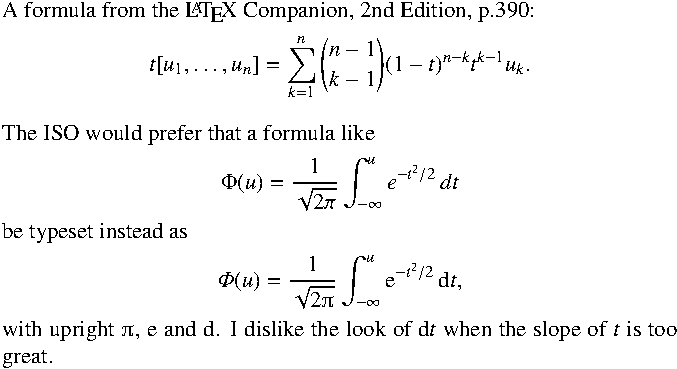
\includegraphics{sample-tx-crop}\]
\begin{itemize}
\item
Complete match between text and math size and weight;
\item first formula much too cramped;
\item upper limit of integral much too close to integral sign;
\item square on $t$ in integrand comes very close to colliding with it;
\item square root in denominator aligned too far right.
\end{itemize}

\vspace{1pc}
\textsc{NEWTXFONTS:}\\
\begin{verbatim}
\usepackage{newtxtext}
\usepackage{newtxmath}
\end{verbatim}
\[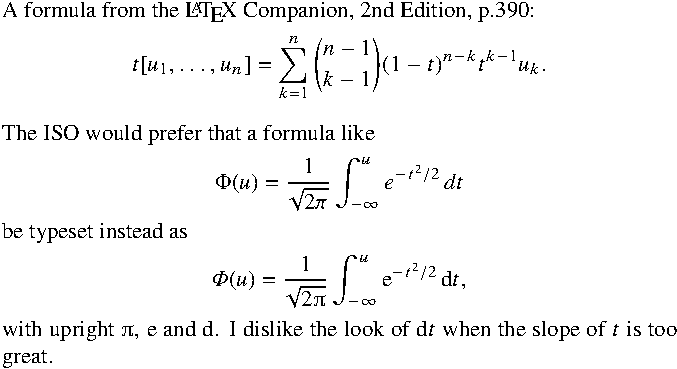
\includegraphics{sample-ntx-crop}\]
\begin{itemize}
\item
Complete match between text and math size and weight;
\item first formula much less cramped;
\item upper limit of integral not too close to integral sign;
\item square not too close to $t$ in exponent;
\item better alignment of square root in denominator.
\end{itemize}

\vspace{1pc}
\textsc{MathTimePro2:}\\
\begin{verbatim}
\usepackage{newtxtext}
\usepackage[lite]{mtpro2}
\end{verbatim}
\[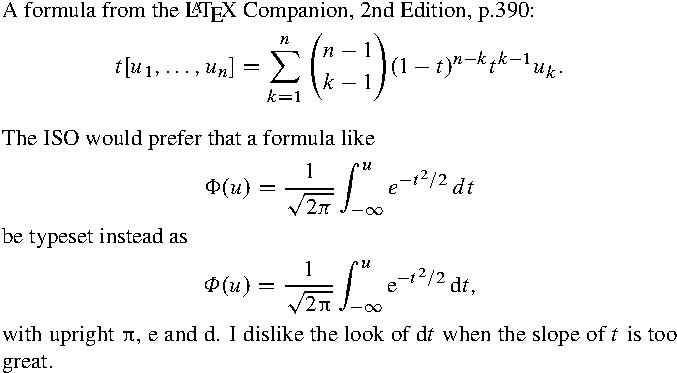
\includegraphics{sample-mtp-crop}\]
\begin{itemize}
\item
Complete match between text and math size and weight;
\item first formula quite spread out;
\item upper limit of integral not too close to integral sign;
\item plenty of space between square and $t$ in exponent.
\end{itemize}

\vspace{1pc}
\textsc{Libertine and MathTimePro2:}\\
\begin{verbatim}
\usepackage{libertine}
\usepackage[T1]{fontenc}
\usepackage[lite]{mtpro2}
\end{verbatim}
\[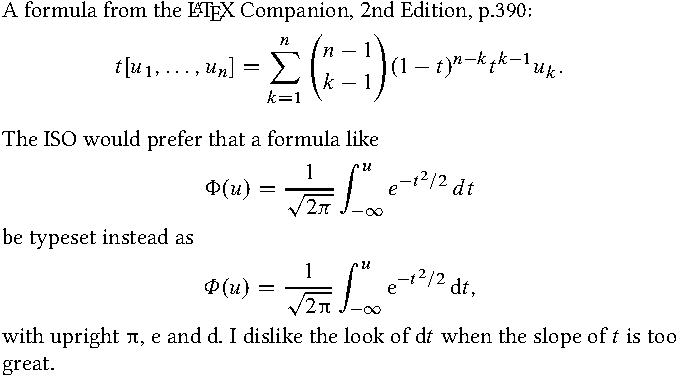
\includegraphics{sample-libmtp-crop}\]
\begin{itemize}
\item
Mismatch of weight between text and math;
\item first formula quite spread out;
\item upper limit of integral not too close to integral sign;
\item plenty of space between square and $t$ in exponent.
\end{itemize}

\vspace{1pc}
\textsc{Libertine and newtxmath:}\\
\begin{verbatim}
\usepackage{libertine}
\usepackage[T1]{fontenc}
\usepackage[libertine]{newtxmath}
\end{verbatim}
\[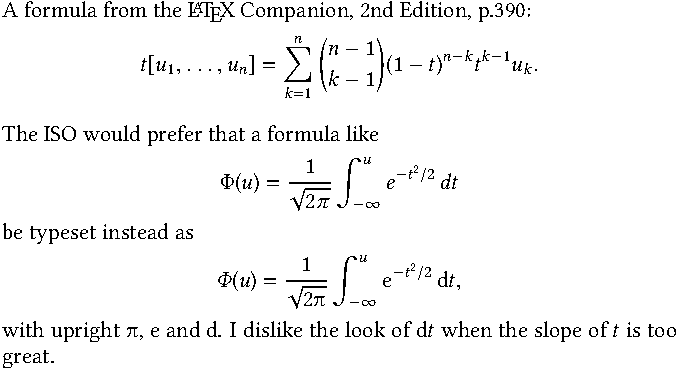
\includegraphics{sample-lib-crop}\]
\begin{itemize}
\item
Very good match between text and math in size and weight;
\item first formula not cramped;
\item upper limit of integral not too close to integral sign;
\item space between square and $t$ in exponent;
\item better alignment of square root in denominator.
\end{itemize}

\vspace{1pc}
\textsc{Mathptmx:}\\
\begin{verbatim}
\usepackage{mathptmx}
\end{verbatim}
\[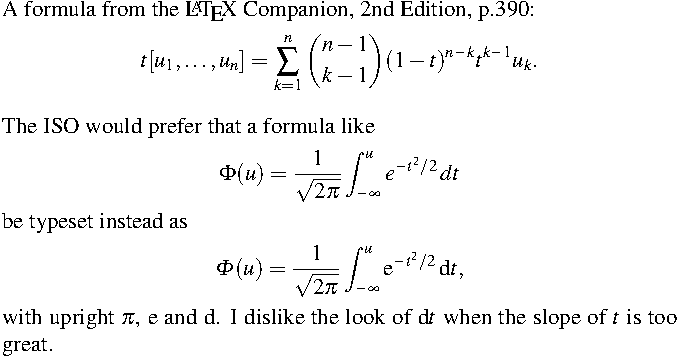
\includegraphics{sample-ptmx-crop}\]
\begin{itemize}
\item
Good match between text and math size and weight, though the summation symbol (from the system {\tt symbol} font) is too small and too dark;
\item first formula well spread;
\item upper limit of integral not too close to integral sign;
\item space between square and $t$ in exponent;
\item there are no upright Greek lowercase letters in this package;
\item good alignment of square root in denominator;
\item infinity symbol not sufficiently large?
\item the package lacks a number of amenities that are present in other packages.
\end{itemize}
\section{Items installed} As well as a collection of PostScript fonts, virtual fonts, font definition files and the central {\tt newtxtext.sty} and {\tt newtxmath.sty} files, the package contains one map file {\tt newtx.map} that must be enabled for the package to function correctly. Its name was changed from {\tt ntx.map} to mirror the package name.) The file \texttt{implementation.pdf} in this distribution provides a manifest of all files installed together with a brief indication of the sources. (This file is somewhat outdated. The file {\tt mathnotes.pdf} adds details about the sources for the math fonts, though it is rather cursory.)

The font files {\tt ntxexmods.pfb} and {\tt ntxbexmods.pfb} were derived from {\tt cmex10.pfb} by FontForgery, thickening the Computer Modern braces to match the weight of the \textsf{txfonts} braces. The pair {\tt ntxexb.pfb} and {\tt ntxbexb.pfb} were similarly derived from {\tt cmsy7.pfb} and {\tt cmex10.pfb} to produce more braces and matching integral signs based on Computer Modern. The {\tt.tfm} files {\tt rtx[b]mio.tfm} are simply unslanted versions of {\tt rtxmi}, from which we construct upright partial derivative symbols.
The last two entries provide us with a way to access custom-encoded versions of {\tt fxlri.pfb} and {\tt fxlbi.map} in order to access some of the unencoded alternate characters---eg, Greek letters, {\tt J.alt} and {\tt v.alt}. The font file \textsf{LibertineTheta-Regular.pfb} was created from the Theta symbol in {\tt fxlri.pfb}, which requires some FontForge help to look correct.

This version contains optical versions of the math italic and symbol fonts at 7\texttt{pt} and 5\texttt{pt}, allowing better rendering in \verb|\scriptstyle| and \verb|\scriptscriptstyle|. 
%\newpage
\section{Changed Math Font Tables}
\subsection{letters}
\fonttable{ntxmi}
\newpage  
\subsection{lettersA}
\fonttable{ntxmia}
\newpage  
\subsection{symbols}
\fonttable{ntxsy}
%\newpage 
 
\subsection{A sample newtx-subs.tex}
You may either copy the entire block below, starting with the line \verb|\begin{...| and ending after the line beginning \verb|\end{|
and pasting it into the top of your document before the \verb|\documentclass...| line, which will allow for easy editing and will write the file to the same folder as your document, or make your own file, omitting those outer two lines.

\begin{verbatim}
\begin{filecontents*}{newtx-subs.tex}
{f}{-3}
{j}{-3}
{p}{-1}
{y}{-1}
{A}{-3}
{B}{-1}
{D}{-1}
{H}{-1}
{I}{-1}
{K}{-1}
{L}{-1}
{M}{-1}
{N}{-0.5}
{P}{-1}
{X}{-1}
{\rho}{-1.5}
{\mu}{-1}
\end{filecontents*}
\end{verbatim}
\subsection*{The {\tt ebgaramond} option to newtxmath}
As {\tt ebgaramond} has an x-height considerably smaller than {\tt newtx}, some amount of scaling is useful to bridge the gap. In making the replacement letters, I increased the size of the EBGaramond letters in math by 5\%, so make some scaling combination for text that compensates for this. The weights of {\tt ebgaramond} used in the substitutions were regular and semibold. This dictates one of the options used for {\tt ebgaramond}.

\textsc{Example preamble not using newtx:}
\begin{verbatim}
\usepackage[lining,semibold,scaled=1.05]{ebgaramond} 
% Latex BOLD renders with ebgaramond semibold 
\usepackage[T1]{fontenc} % best for Western European languages
\usepackage[varqu,varl]{inconsolata}% a typewriter font for \mathtt
\usepackage{amsmath}% must be loaded before amsthm, if using
\usepackage{amsthm}% must be loaded before newtxmath
\usepackage[ebgaramond,vvarbb,subscriptcorrection,alth]{newtxmath} % STIX Bbb
% Option alth replaces math h with a more traditional shape
\usepackage{bm}% load after all math to give access to bold math
\end{verbatim}
\textsc{Same preamble using newtx:}
\begin{verbatim}
\usepackage[T1]{fontenc} % best for Western European languages
\usepackage[varqu,varl]{inconsolata}% a typewriter font for \mathtt
\usepackage[ebgaramond,semibold,textscale=0,vvarbb,subscriptcorrection,amsthm,alth]{newtx}
\usepackage{bm}% load after all math to give access to bold math
\end{verbatim}
%}

\section{Changes to math character names in version 1.72}
The names of some math characters containing a colon had become inconsistent with {\tt unicode-math} and the {\tt mathtools} package. Revision 1.72 (2023) of {\tt newtx} harmonizes the commands for colon-related math glyphs with the revisions made in 2022 in the {\tt mathtools} package---the last column below shows the new names used for such glyphs in {\tt newtx} that are also in {\tt mathtools}. The changes are consistent with the unicode-math command names.

\begin{center}Math colon symbols in newtxmath and mathtools (MT)\\ \vspace{6pt}
  \begin{tabular}{@{} ccccccc @{}}
    \toprule
    Symbol &  u+ & unicode-math & txfonts &  legacy newtx & legacy MT & newtx/MT \\ 
    \midrule
    $\colonapprox$ &  • & • & \verb|\colonapprox| & \verb|\colonapprox| & \verb|\colonapprox| & \verb|\colonapprox| \\ 
     $\colonsim$ &  • & •  & \verb|\colonsim| &  \verb|\colonsim| & \verb|\colonsim| & \verb|\colonsim|  \\ 
    $\Colonapprox$ &  • & • & \verb|\Colonapprox| &  \verb|\Colonapprox| & \verb|\Colonapprox| & \verb|\Colonapprox| \\ 
    $\Colonsim$ &  • & •  & \verb|\Colonsim| & \verb|\Colonsim| &  \verb|\Colonsim| & \verb|\Colonsim| \\ 
    $\coloneq$ &  2254 & \verb|\coloneq|  &\verb|\coloneqq| & \verb|\coloneq| & \verb|\coloneqq| & \verb|\coloneq| \\ 
    $\eqcolon$ &  2255 & \verb|\eqcolon|  &\verb|\eqqcolon| &  \verb|\eqcolon| & \verb|\eqqcolon| & \verb|\eqcolon| \\ 
    $\colondash$ &  • & •  &\verb|\coloneq| & • &  \verb|\coloneq| & \verb|\colondash| \\ 
    $\dashcolon$ &  2239 & \verb|\dashcolon|  &\verb|\eqcolon| &  • & \verb|\eqcolon| & \verb|\dashcolon| \\ 
    $\Coloneq$ &  2A74 & \verb|\Coloneq|  & \verb|\Coloneqq| & \verb|\Coloneqq| & \verb|\Coloneqq| & \verb|\Coloneq| \\ 
    $\Eqcolon$ &  • & •  &\verb|\Eqqcolon| &  \verb|\Eqqcolon| & \verb|\Eqqcolon| & \verb|\Eqcolon| \\ 
    $\Colondash$ &  • & •  & \verb|\Coloneq| & \verb|\Coloneq| & \verb|\Coloneq| & \verb|\Colondash| \\ 
    $\Dashcolon$ &  • & •  & \verb|\Eqcolon| & \verb|\Eqcolon| & \verb|\Eqcolon| & \verb|\Dashcolon| \\ 
    \bottomrule
  \end{tabular}
\end{center}


For users with existing documents using any of the symbols in the last four rows, the legacy {\tt newtx} commands are aliased to the new commands. Unless the commands \verb|\Coloneqq|, \verb|\Eqqcolon|, \verb|\Coloneq| and \verb|\Eqcolon| have already been defined, the effect is the same as 
\begin{verbatim}
\let\Coloneqq\Coloneq
\let\Eqqcolon\Eqcolon
\let\Coloneq\Colondash
\let\Eqcolon\Dashcolon
\end{verbatim}
\section{Appendix 1: Changes made in version 1.5}
\begin{itemize}
\item
The large delimiters have been modified so match the heights in common usage by \texttt{cmex10} and other packages. (Those formerly used by \texttt{newtxmath} were somewhat shorter, resulting in unexpected behavior of \verb|\Big|, \verb|\bigg|, etc.)
\item
The integrals used in previous versions have been discarded and replaced by an upright and a slanted form, the latter being the default. The option {\tt upint} switches to the upright form. (The former option {\tt cmintegrals} now has no effect.) Integrals are of three types: small, textstyle and displaystyle. Each size is available in twelve variants. Assuming slanted (the default) is selected, there are 36 regular-weight forms:
\setlength{\extrarowheight}{8pt}
\begin{center}
  \begin{tabular}{@{} llll @{}}
    \toprule
     Small && Text, Display& \\ 
    \midrule
$\smallint$  & \verb|$\smallint$|& $\int$, $\displaystyle{\int}$& \verb|$\int$|\\ 
$\smalliint$  & \verb|$\smalliint$|& $\iint$, $\displaystyle{\iint}$&\verb|$\iint$|\\ 
$\smalliiint$  & \verb|$\smalliiint$|& $\iiint$, $\displaystyle{\iiint}$& \verb|$\iiint$|\\ 
$\smalliiiint$  & \verb|$\smalliiiint$|& $\iiiint$, $\displaystyle{\iiiint}$& \verb|$\iiiint$|\\ 
$\smalloint$  & \verb|$\smalloint$|& $\oint$, $\displaystyle{\oint}$& \verb|$\oint$|\\ 
$\smalloiint$  & \verb|$\smalloiint$|& $\oiint$, $\displaystyle{\oiint}$& \verb|$\oiint$|\\ 
$\smalloiiint$  & \verb|$\smalloiiint$|& $\oiiint$, $\displaystyle{\oiiint}$& \verb|$\oiiint$|\\ 
$\smallfint$  & \verb|$\smallfint$|& $\fint$, $\displaystyle{\fint}$& \verb|$\fint$|\\ 
$\smallsqint$  & \verb|$\smallsqint$|& $\sqint$, $\displaystyle{\sqint}$& \verb|$\sqint$|\\ 
$\smallsumint$  & \verb|$\smallsumint$|& $\sumint$, $\displaystyle{\sumint}$& \verb|$\sumint$|\\ 
$\smallvarointclockwise$  & \verb|$\smallvarointclockwise$|& $\varointclockwise$, $\displaystyle{\varointclockwise}$& \verb|$\varointclockwise$|\\ 
$\smallointctrclockwise$  & \verb|$\smallointctrclockwise$|& $\ointctrclockwise$, $\displaystyle{\ointctrclockwise}$& \verb|$\ointctrclockwise$|\\ 
    \bottomrule
  \end{tabular}
\end{center}
\item  The overly small delimiters ([\{ in Times are no longer used in math mode, being replaced by bigger versions. The former option {\tt bigdelims} no longer has any effect.
\item There is a new option {\tt smallerops} which chooses smaller renditions (20\% smaller in displaystyle, 10\% smaller in textstyle) of the {\tt bigoperators}:
\begin{verbatim}
\bigsqcup
\bigodot
\bigoplus
\bigotimes
\sum
\prod
\bigcup
\bigcap
\biguplus
\bigwedge
\bigvee
\bigcupdot
\bigcapplus
\bigsqcupplus
\bigsqcapplus
\bigsqcap
\bigtimes
\coprod
\end{verbatim}
\item The dot accents are now taken from a slightly larger series, making available \verb|\dot|, \verb|\ddot|, \verb|\dddot| and \verb|\ddddot|. For best horizontal alignment with other accents, choose the option {\tt timesmathacc} when loading {\tt newtxmath}.
\item New accents have been added and the old vector accent has been replaced. The new accents are:
\verb|\vec|$\quad\vec{}$\\
\verb|\lvec|$\quad\lvec{}$\\
\verb|\lrvec|$\quad\lrvec{}$\\
\verb|\harpoonacc|$\quad\harpoonacc{}$\\
\verb|\lharpoonacc|$\quad\lharpoonacc{}$\\
\verb|\lrharpoonacc|$\quad\lrharpoonacc{}$\\
\verb|\barbar|$\quad\barbar{}$\\
\verb|\bartilde|$\quad\bartilde{}$\\
\verb|\barhat|$\quad\barhat{}$\\
\verb|\tildebar|$\quad\tildebar{}$\\
\verb|\tildetilde|$\quad\tildetilde{}$\\
\verb|\tildehat|$\quad\tildehat{}$\\
\verb|\hatbar|$\quad\hatbar{}$\\
\verb|\hattilde|$\quad\hattilde{}$\\
\verb|\hathat|$\quad\hathat{}$\\
\item New glyphs: (B denotes bigger, S denotes smaller)\\
\verb|\cdotB| $\quad\cdotB$ (cf. \verb|\cdot| $\quad\cdot$)\\
\verb|\cdotBB| $\quad\cdotBB$\\
\verb|\circS| $\quad\circS$ (cf. \verb|\circ| $\quad\circ$)\\
\verb|\bulletS| $\quad\bulletS$ (cf. \verb|\bullet| $\quad\bullet$)\\
\verb|\bulletSS| $\quad\bulletSS$\\
\verb|\bulletSSS| $\quad\bulletSSS$\\
\verb|\primeS| $\quad\primeS$ (cf. \verb|\prime| $\quad\prime$)\\
\item New macros \verb|\setSYdimens| and \verb|\setEXdimens| allow experts to modify some math font dimensions.
\end{itemize}
\def\jj{\mkern-3mu j}

\section{Appendix 2: Changes made in version 1.60}
Versions of {\tt newtx}  dated from September, 2019 (1.60 for {\tt newtxmath} make some quite substantial changes, mostly to math mode. 
\section{Goals}
Spurred by work of Ross Moore to provide means of generating archivable pdf using {\tt pdflatex}, the main goal was to change {\tt newtx} and {\tt newpx} to meet the requirements for satisfying the {\tt PDF/A-1b} standards by using an appropriate preamble involving the {\tt pdfx} package and other unicode mapping files. Making these  changes  gave me the opportunity to organize the source files to make them more manageable in  future revisions. 

A further goal whose time seemed ripe was to rework the  spacing of math letters, both Roman and Greek, so they behaved better in superscripts and subscripts. This did not turn out to be so easy. The problem is illustrated by math italic j. If you don't give it enough extra space on the left, it will likely collide with the D in rendering \verb|$D^j$|. On the other hand, if you do give it enough space on the left, it will look bad as a  subscript, appearing too far right. 

A final goal was to make better use of the remaining space in some of the math fonts by placing some math alphabets in them, avoiding perhaps a waste of those precious sixteen math families.
\section{The important changes}
The following changes were made to both {\tt newtx} and {\tt newpx}.
\subsection{Archivability}
Some of the individual font files from which the math fonts are built turned out to have some fairly minor structural issues. These have all been corrected. The more major issue was the lack of unicode mapping for all characters in the fonts. For the symbol and math extension fonts, this issue was largely solved by Ross Moore's {\tt glyphtounicode} files that are now accessible as part of TeXLive and MiKTeX. The main problem was the math alphabets like math italic, bold math italic, upright Greek and slanted Greek, all of which have now been assigned their own unicode points. For all of these, I constructed new fonts using unicode names for the glyphs, then made \textsf{fontinst} scripts that renamed those unicode values to the original simple names as used in the encoding files so that I could use my old encoding and adjustment files. This exercise has now been carried out for {\tt newtxmath}, {\tt newpxmath}, {\tt newtxmath/libertine}, {\tt newtxmath/cochineal}, {\tt newtxmath/stix2}, {\tt newtxmath/xcharter} and {\tt newtxmath/erewhon.} Each of these can now be considered to have an ``enhanced'' status that allows them to share all the new assets described below. 
 The other packages which may be specified as an option to {\tt newtxmath} (e.g., {\tt baskervaldx, baskervillef}) must be considered for the moment to be ``unenhanced'' and able to share only some of the new assets. In particular, only the enhanced items can generate archivable pdf. 

Also modified were the {\tt sups} fonts in {newtxtext}, where the main issue was unicode mapping. Superior numbers and some superior letters do have assigned unicode values, but in may cases a more creative approach was needed, and provided once again by Ross Moore. I rebuilt the superior font files using those unicode names, solving that particular problem.

Here is a sample  preamble showing the elements you will need to specify to generate a pdf satisfying the PDF/A-1b standards, as verified by Adobe Acrobat Pro. (Other verification processes may yield different outcomes.)


\begin{verbatim}
\documentclass[noamsfonts]{amsart} % save 2 math families 
%\pdfcompresslevel=0 %Set this only if are going to debug the pdf
%\pdfgentounicode=1 %These to lines no longer needed--LaTeX does it.
%\input glyphtounicode.tex 
\usepackage{pdfx} % v 1.6.4 or higher
\InputIfFileExists{glyphtounicode-cmr.tex}{}{} 
\InputIfFileExists{glyphtounicode-ntx.tex}{}{}
\usepackage{newtxtext} %T1 is default encoding
\usepackage[scaled=0.95]{inconsolata}  % typewriter
\usepackage[leqno]{amsmath} 
\usepackage{amsthm}
\usepackage[vvarbb]{newtxmath} % vvarbb gives STIX Bbb
\end{verbatim} 


\subsection{Glyph spacing changes} \textbf{(For enhanced packages only)}I reworked the math italics to improve the rendering of some  superscripts. This affects (a)  parentheses, brackets and braces to inhibit clashes; (b) glyphs like j, f, p, y, \verb|\rho|,  \verb|\beta| and  \verb|\mu| where a long tail could pose problems intersecting with other glyphs; (c) glyphs like such as D, Q and \verb|\Phi| that are round on the right, where interference is most likely to occur with a superscript. Increasing the left side-bearing of j, etc., helps with superscripts but creates an ugly gap when used as subscripts.  


 The {\tt subscriptcorrection} option to {\tt newtxmath} has been corrected and enhanced  so that it now offers a partial solution the subscript spacing problem. I regret that this option is incompatible with {\tt xy-pic}, both depending on making \verb|_| an active character. {\tt Newtxmath}  will detect if the {\tt xy} package is loaded and disable {\tt subscriptcorrection} if so. You would have to correct such issues by manually inserting a negative \verb|\mkern|. For example, you might put in your preamble something like
 \begin{verbatim}
\def\jj{\mkern-3mu j}
\end{verbatim}
and then use \verb|$x_{\jj}$| instead of \verb|$x_j$|, turning $x_j$ into $x_{\jj}$.

There are also interactions with {\tt pstricks} that have to be worked around because {\tt subscriptcorrection} redefines \verb|_| as an active character, as do parts of {\tt pstricks}. In particular, the {\tt pstricks} short forms for macros like \verb|\tbput| and \verb|\nbput| for attaching labels beneath node connections must be avoided.


If you do enable {\tt subscriptcorrection}, there is a default correction table in the {\tt sty} file, but the sty file also looks for a file named, e.g., {\tt newtx-subs.tex} if you are using the {\tt newtx} default math letters. There is already such a file located in the {\tt newtx} distribution in the \verb|/tex/latex/| folder. If you wish to make changes to this file, copy the file to your home TeX folder where it will be found by TeX before the one in the distribution. The entries in the file are lines like
\begin{verbatim}
{j}{-3}
\end{verbatim}
each of which will have the same effect as the above macro if the first item in the subscript is j. You can also specify Greek letters with lines like
\begin{verbatim}
{\beta}{-1.5}
\end{verbatim}
The complete list of file names recognized for specifying subscript corrections is:
\begin{verbatim}
newtx-subs.tex
newtx-libertine-subs.tex
newtx-xcharter-subs.tex
newtx-cochineal-subs.tex
newtx-baskervillef-subs.tex
newtx-stickstoo-subs.tex
newtx-garamond-subs.tex
newtx-ebgaramond-subs.tex
newtx-baskervald-subs.tex
newtx-erewhon-subs.tex
newtx-minion-subs.tex
newtx-nc-subs.tex
newtx-ncf-subs.tex
newtx-noto-subs.tex
newtx-notosans-subs.tex
\end{verbatim}

\subsection{New glyphs added} \textbf{(For enhanced packages only)} Math family 1 {\tt (letters)} has been extended from 128 slots to 256, retaining the {\tt OML} encoding of the first 128. Most of additional slots have been allocated to a script font from the old STIX collection and an upright modification of that font.
By default, \verb|$\mathscr{F}$| will produce $\mathscr{F}$.\\
$\bullet$ option {\tt uprightscript} changes the output to {\usefont{OML}{ntxmi}{m}{it}\char201}.\\
In both cases, there are full upper-case and lower-case and {\tt dotlessi}, {\tt dotlessj}. To insert the latter, you can write either \verb|$\mathscr{\imath}$| or \verb|$\imathscr$|, rendered as $\mathscr{\imath}$ in the slanted script case. 

There are in fact two additional macros, \verb|\mathslscr| (slanted script) and \verb|\mathuscr| (upright script) that may be used. By default, \verb|\mathscr| is \verb|\let| to \verb|\mathslscr|, but, under option {\tt uprightscript}, \verb|\mathscr| is \verb|\let| to \verb|\mathuscr|.

The secondary letters font {\tt (lettersA)} and math family 2 {\tt(symbols)} have been rearranged. The first of these continues to have a Fraktur alphabet, but it a modification of its original one, having wider vertical stems and a blacker appearance more in keeping with the weight of Times. {\tt Dotlessi} and {\tt dotlessj} have been added and can be specified in math mode by \verb|$\imathfrak$| and \verb|$\jmathfrak$|---\verb|$\mathfrak{\imath}$| also works. There are in addition two subsidiary Bbb alphabets in {\tt lettersA}, specified by the respective options {\tt varbb}, {\tt vvarbb}, and there are corresponding {\tt dotlessi}, {\tt dotlessj} activated by \verb|$\imathbb$|, \verb|$\jmathbb$|, which always render as $\imathbb$, $\jmathbb$ no matter the choice of which Blackboard Bold Alphabet. If you select one of the options {\tt varbb}, {\tt vvarbb}, you will have Bbb digits 0..9 using, e.g., \verb|$\mathbb{1}$| to get~$\vvmathbb{1}$. With both options, the arguments \verb|\imath|, \verb|\jmath| will render as expected, as are all upper and lower case letters.


Among the new symbols added are:\\
$\bullet$ \verb|\hslash|, \verb|\hbar|, \verb|\lambdaslash|, \verb|\lambdabar|, \verb|\Zbar|, \verb|\Angstrom| are now constructed from the native glyphs, but only in the enhanced families.\\
$\bullet$ Euler's constant \verb|$\Euler$| ($\Euler$).\\
$\bullet$ Hermitian transpose \verb|\hermtransp| or \verb|\htransp| is used like \verb|$\mathbf{A}^{\htransp}$| ($\mathbf{A}^{\htransp}$). This usage is similar to simple transpose \verb|$\mathbf{A}^{\transp}$| ($\mathbf{A}^{\transp}$).\\
$\bullet$ Independence (in the probabilistic sense) can use \verb|\Perp|, $\Perp$, and there is a new \verb|\nPerp|, $\nPerp$ for its negation.

\subsection{Adaptive vector accent} The \LaTeX\ macro \verb|\overrightarrow| provides a right arrow with adaptive width, but not matching the vector head of {\tt newtxmath}. Likewise, the {\tt esvect} provides a similar service with a choice of vector heads, none of which match {\tt newtxmath}. I've added code to provide a matching adaptive vector accent and which uses the same macro name, \verb|\vv|, as {\tt esvect}.

For a comparison of these vector accents, \verb|$\vec{XY} \vv{XY} \overrightarrow{XY}$| renders as\\ 
$\vec{XY} \vv{XY} \overrightarrow{XY}$.\\ 
$\bullet$ \verb|$\vv{AB}$|  renders as $\vv{AB}$.\\ 
$\bullet$ \verb|$\vv*{AB}{x}$| renders as $\vv*{AB}{x}$. This provides better horizontal spacing of subscripts than \verb|$\vv{AB}_{x}$|, $\vv{AB}_{x}$.\\
$\bullet$  You can also do \verb|$\vv*{AB}{\vv{CD}}$|, which  renders as $\vv*{AB}{\vv{CD}}$.\\
$\bullet$ You can change the vertical space between the arrow and the accentee by means of the package option {\tt vecsep}, whose default value is {\tt .25ex}.

\subsection{A widebar accent to complement widehat and  widetilde}
The \verb|\widebar| macro added to version 1.7 came to me via Murray Eisenberg. The original version by Hendrik Vogt  was the subject  of considerable discussion on {\tt stackexchange} a few years ago. It  handles very cleverly issues of width, superscript placement and skew. For example: \verb|$\widebar{AB}^C$| gives $\widebar{AB}^C$ and \verb|$\widebar{AB^C}$| gives $\widebar{AB^C}$.
\subsection{Miscellaneous Changes}
\begin{itemize}
\item
The superior letters fonts in {\tt newtx} 
have been extended and all glyphs now have appropriate unicode mappings.
\item
The AMS fonts replacement {\tt ntxsym} corrects the former misplacement of \verb|\kbbb|, \verb|\daleth|, \verb|\circledR| and \verb|\circledS|.)
\end{itemize}


%for {\tt newtx}
%\subsection{Operatorname issues}
%For some of the text fonts supported by {\tt newtx}, an {\tt OT1} version of the text fonts has been constructed with Greek capital letters in the first eleven slots, just as in Computer Modern, and some older TeX constructs depend on that. In those cases, even if you set {\tt T1} as your text font encoding before loading {\tt newtxmath} or {\tt newtx}, the operator font will be set to the {\tt OT1} version, not the {\tt T1} version. (You may prevent this by specifying option {\tt noOT1} to {\tt newtxmath} or {\tt newtx}.) Using the {\tt OT1} encoded operators font should not be a problem unless you wish to use accented characters in some operator names. This is the case in Spanish and Portuguese, and possibly other languages. One solution could be to define the affected operators individually with commands like
%\begin{verbatim}
%\DeclareMathOperator{\mIn}{\text{{\fontencoding{T1}\selectfont m\'in}}}
%\end{verbatim}
%making use of  the {\tt amsmath} \verb|\text| macro, which gives you proper scaling in scriptstyle and scriptscriptstyle as well.
\makeatletter
%\expandafter\show\csname ver@newtx.sty\endcsname
\@ifundefined{ver@newtx.sty}{\end{document}}{\makeatother}
%
%\show\nustyle
\subsection{The stacked fraction macro}
Having collected a lot of data about the text fonts it supports, it seemed worthwhile  to construct in {\tt newtx} a macro that would work for most of those fonts: 
\verb|\textsfrac[1]{17}{32}| renders in {\tt newtxtext} as \textsfrac[1]{17}{32}
 and \verb|\textsfrac{9}{64}| as \textsfrac{9}{64}. Compare these with output from the diagonal fraction macro 
 \verb|\textfrac|: \textfrac[1]{17}{32}, \textfrac{9}{64}.  Note: \verb|\textsfrac| is not available unless you load via {\tt newtx.sty}.

There are four options with which you may control the layout of the fractional part.
\begin{itemize}
\item
{\tt sfracvcenter} controls the vertical center of the fraction bar.
\item{\tt sfracbarthick} controls its thickness.
\item{\tt sfracvspacing} controls the vertical space above and below the fraction bar.
\item{\tt sfracscaling} controls the size of the figures in the fraction.
\end{itemize}
The last of these is just a number like .85 by which to scale the denominator figures used in the construction. The first three items may be specified in either {\tt em} units or in {\tt ex} units. If you use a number greater than 6, it is interpreted as a multiple of an {\tt em} (recall that for most fonts, and certainly for those supported by {\tt newtx}, 100{\tt em} is equal to 1{\tt pt} if you are processing at 10{\tt pt}. On the other hand, 1{\tt ex} is the height of the letter x in the current text font. If you specify a number less than 6, it is interpreted in {\tt ex} units.

\end{document}